\documentclass[a4paper,10pt,DIV=15,mpinclude=true]{scrartcl}
\usepackage[xetex]{graphicx}
\usepackage{amsmath,amsthm}
\usepackage[usenames,dvipsnames,svgnames,table]{xcolor}

\linespread{1.5}
\textwidth=480pt

\usepackage{hyperref}
\usepackage[T1]{fontenc}

% Comment out the next three lines to revert to Times New Roman
\usepackage{pxfonts}
\usepackage[scaled=0.86]{berasans}
\usepackage[scaled=0.96]{inconsolata}

\usepackage{afterpage}
\usepackage{verbatimbox}

% Change the style of the captions and the headers
\usepackage[normal,bf,labelsep=quad]{caption}
\usepackage{subcaption}
\setkomafont{caption}{\sffamily}
\setkomafont{disposition}{\bfseries}

% Macro for finding figures
\graphicspath{{/Users/desislava/Documents/GitHub/eems/Documentation/Figures/}}


\begin{document}

EEMS is a program to analyze and visualize spatial population structure from geo-referenced genetic samples. EEMS uses the concept of \textit{effective migration} to model the relationship between genetics and geography, and it outputs an estimated effective migration surface (hence, EEMS) -- a visual representation of population structure that highlights potential regions of higher-than-average and lower-than-average historic gene flow.

This EEMS implementation uses Eigen for linear algebra computations and Boost for random number generation and the habitat geometry. (The habitat is assumed to be a (possibly irregular) closed polygon without holes; see Section \ref{sec:habitat}.) The Eigen template library can be downloaded from \url{http://eigen.tuxfamily.org}, and the Boost libraries can be downloaded from \url{http://www.boost.org}. EEMS has been tested with Eigen 3.2.2 and Boost 1\_57.

\section{The input files}

There are three data input files plus a parameter input file. The data input files should be in the same directory, and the description below assumes that \textit{datapath} specifies their location.

For SNP data, the input files are:
\begin{itemize}
  \item \textit{datapath}.diffs: the matrix of average pairwise genetic differences. (This matrix can be computed with {\tt bed2diffs} if the dataset is already in plink binary format.)
  \item \textit{datapath}.coord: the sample coordinates (two coordinates per sample, one sample per line)
  \item \textit{datapath}.outer: the habitat coordinates (as a sequence of vertices that outline a closed polygon; see Section \ref{sec:habitat} for details and some examples.)
\end{itemize}

For microsatellite data, the input files are:
\begin{itemize}
  \item \textit{datapath}.sites: the matrix of allele copies (one sample per line, $2L$ alleles per sample, where $L$ is the number of microsatellites; missing alleles can be specified by any negative number.)
  \item \textit{datapath}.coord: as described above for SNP data.
  \item \textit{datapath}.outer: as described above for SNP data.
\end{itemize}

\section{The habitat} \label{sec:habitat}

The habitat is represented as a ring (a polygon without holes), with vertices listed counterclockwise in the file \textit{datapath}.outer, with one vertex per line. See Figure \ref{fig:habitat-examples} for examples.

The vertices of the population graph (the demes) will fall inside the habitat by construction. However, EEMS will not check that the sampling locations fall inside the habitat -- instead, each sample will be assigned to the closest deme. Therefore, the user should specify a habitat that is sufficiently large to cover all sampling locations.

\begin{myverbbox}{\habitatA}
Input habitat: 
  POLYGON((0 0,0 6,12 6,12 0))
Corrected habitat: 
  POLYGON((0 0,0 6,12 6,12 0,0 0))
  
  
\end{myverbbox}
\begin{myverbbox}{\habitatB}
Input habitat: 
  POLYGON((0 0,0 6,12 6,12 0,0 0))
    


  
\end{myverbbox}
\begin{myverbbox}{\habitatC}
Input habitat: 
  POLYGON((0 0,12 0,12 6,0 6,0 0))
Corrected habitat: 
  POLYGON((0 0,0 6,12 6,12 0,0 0))  


\end{myverbbox}
\begin{myverbbox}{\habitatD}
Input habitat: 
  POLYGON((0 0,2 3,0 6,12 6,10 3,
           12 0,0 0))
  

  
\end{myverbbox}
 
\afterpage{
\begin{figure}

\begin{subfigure}[t]{\textwidth}
\centering
\begin{tabular}{p{2.7in}c}
\habitatA&
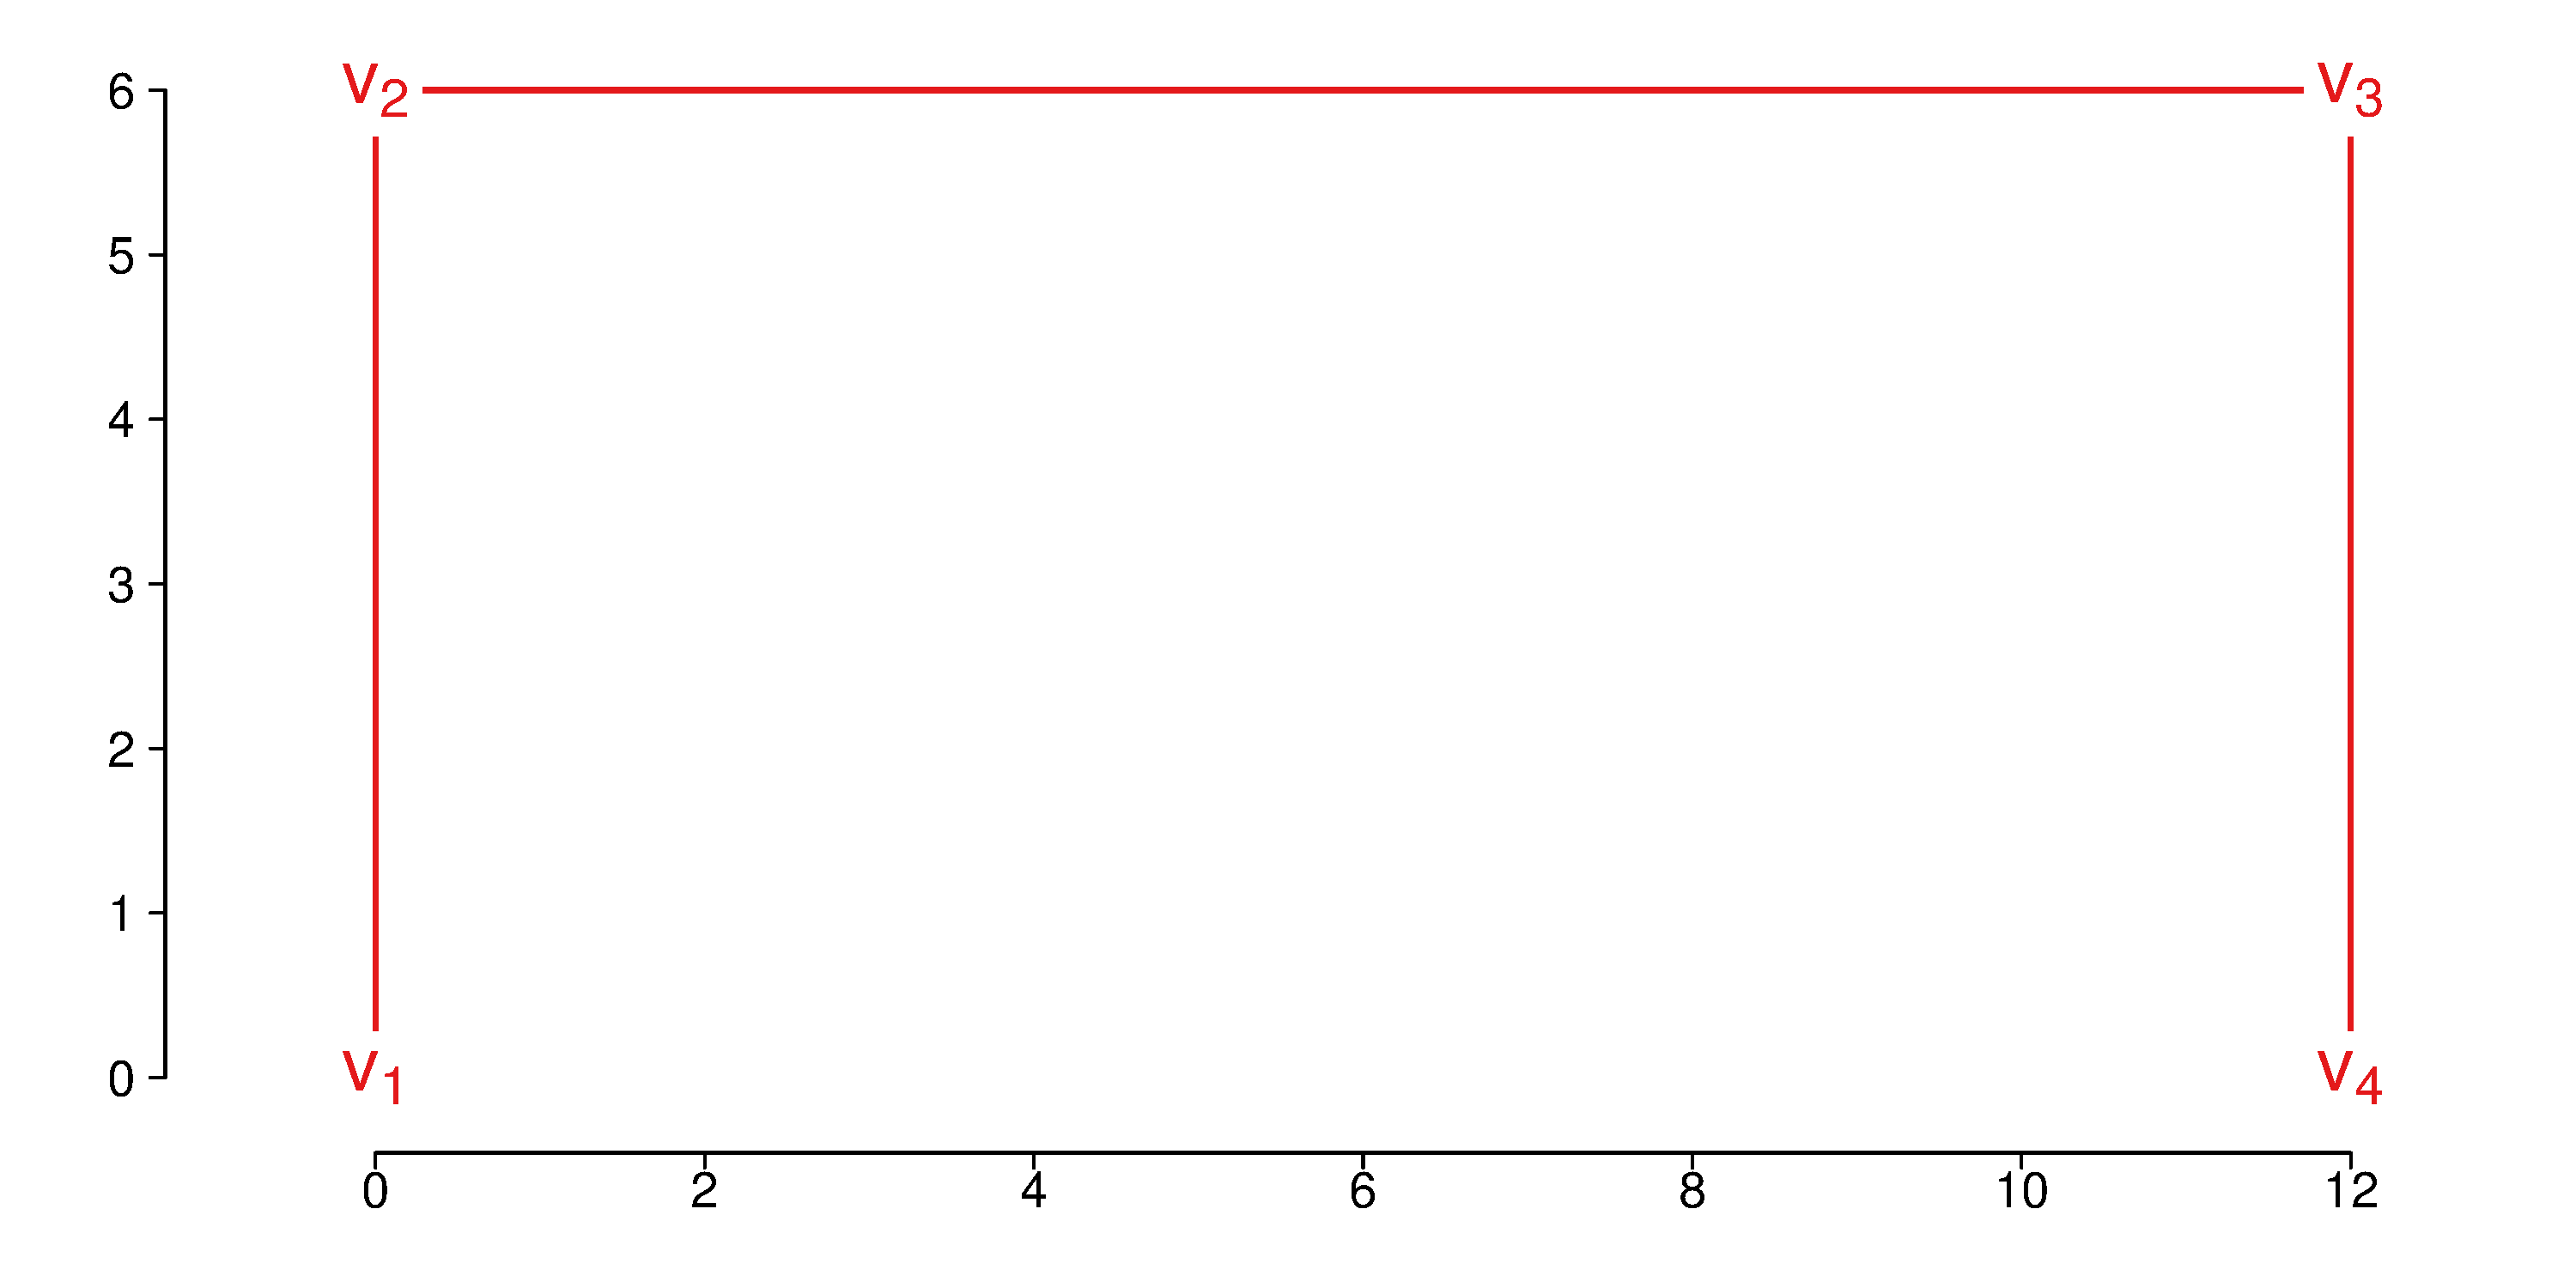
\includegraphics[height=1.7in]{rectangular-habitat-choose_grid01.png}
\end{tabular}
\caption{}
\end{subfigure}

\vspace{20pt}

\begin{subfigure}[t]{\textwidth}
\centering
\begin{tabular}{p{2.7in}c}
\habitatC&
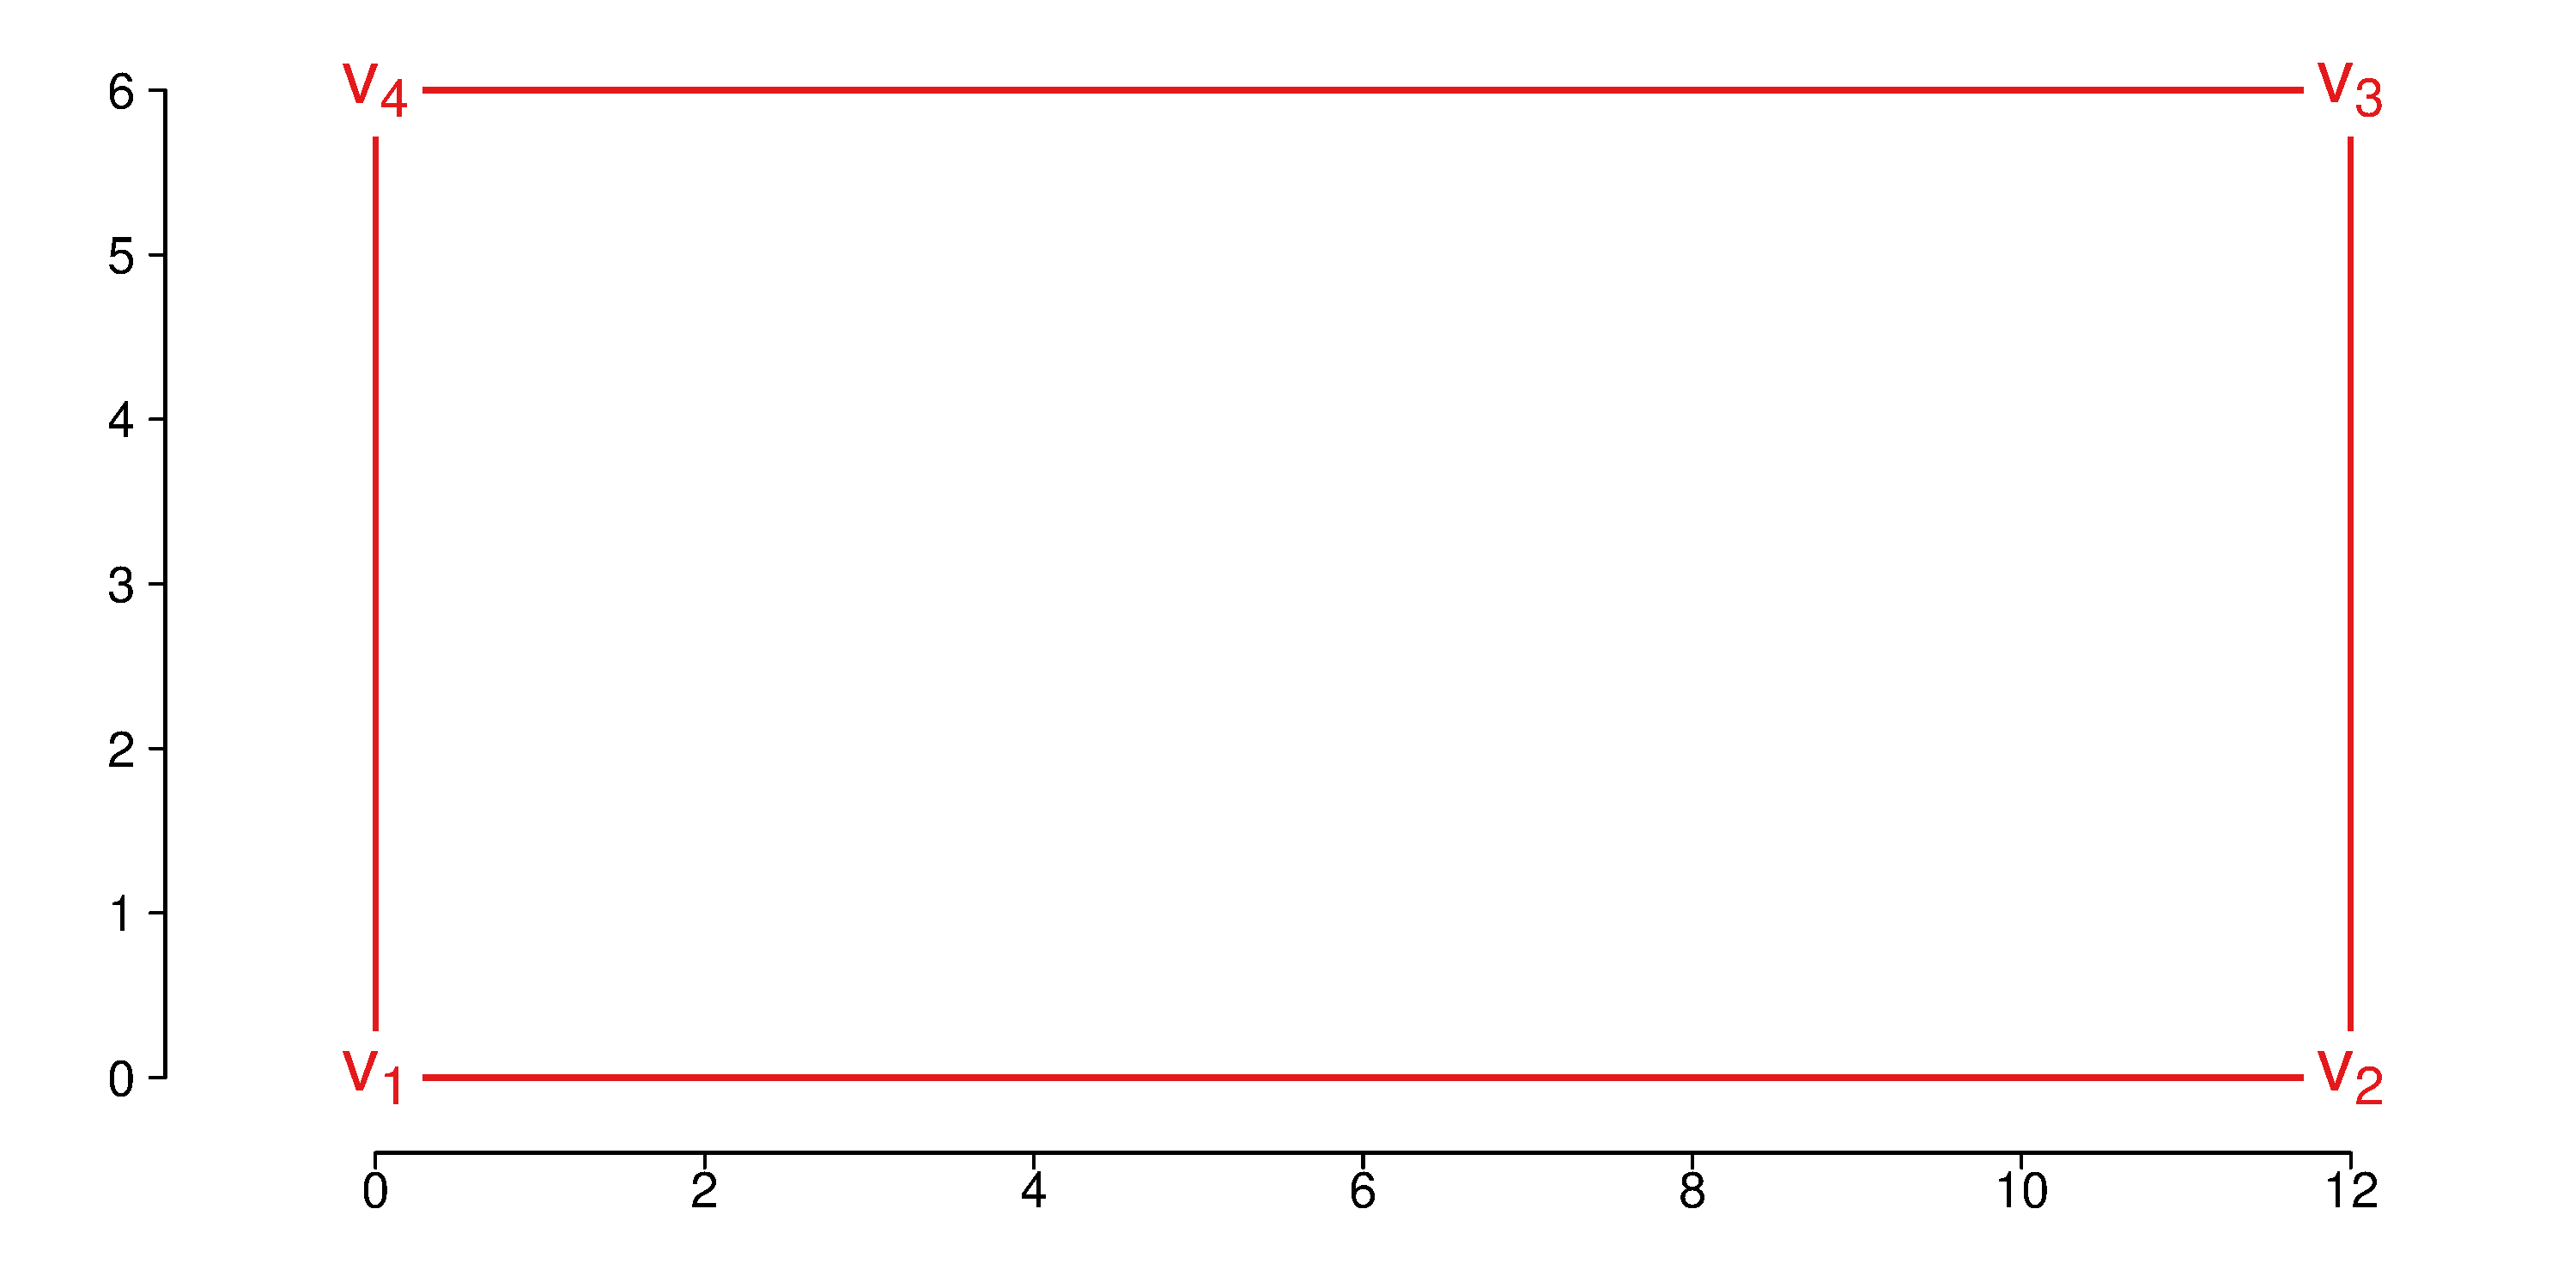
\includegraphics[height=1.7in]{rectangular-habitat-choose_grid03.png}
\end{tabular}
\caption{}
\end{subfigure}

\vspace{20pt}

\begin{subfigure}[t]{\textwidth}
\centering
\begin{tabular}{p{2.7in}c}
\habitatD&
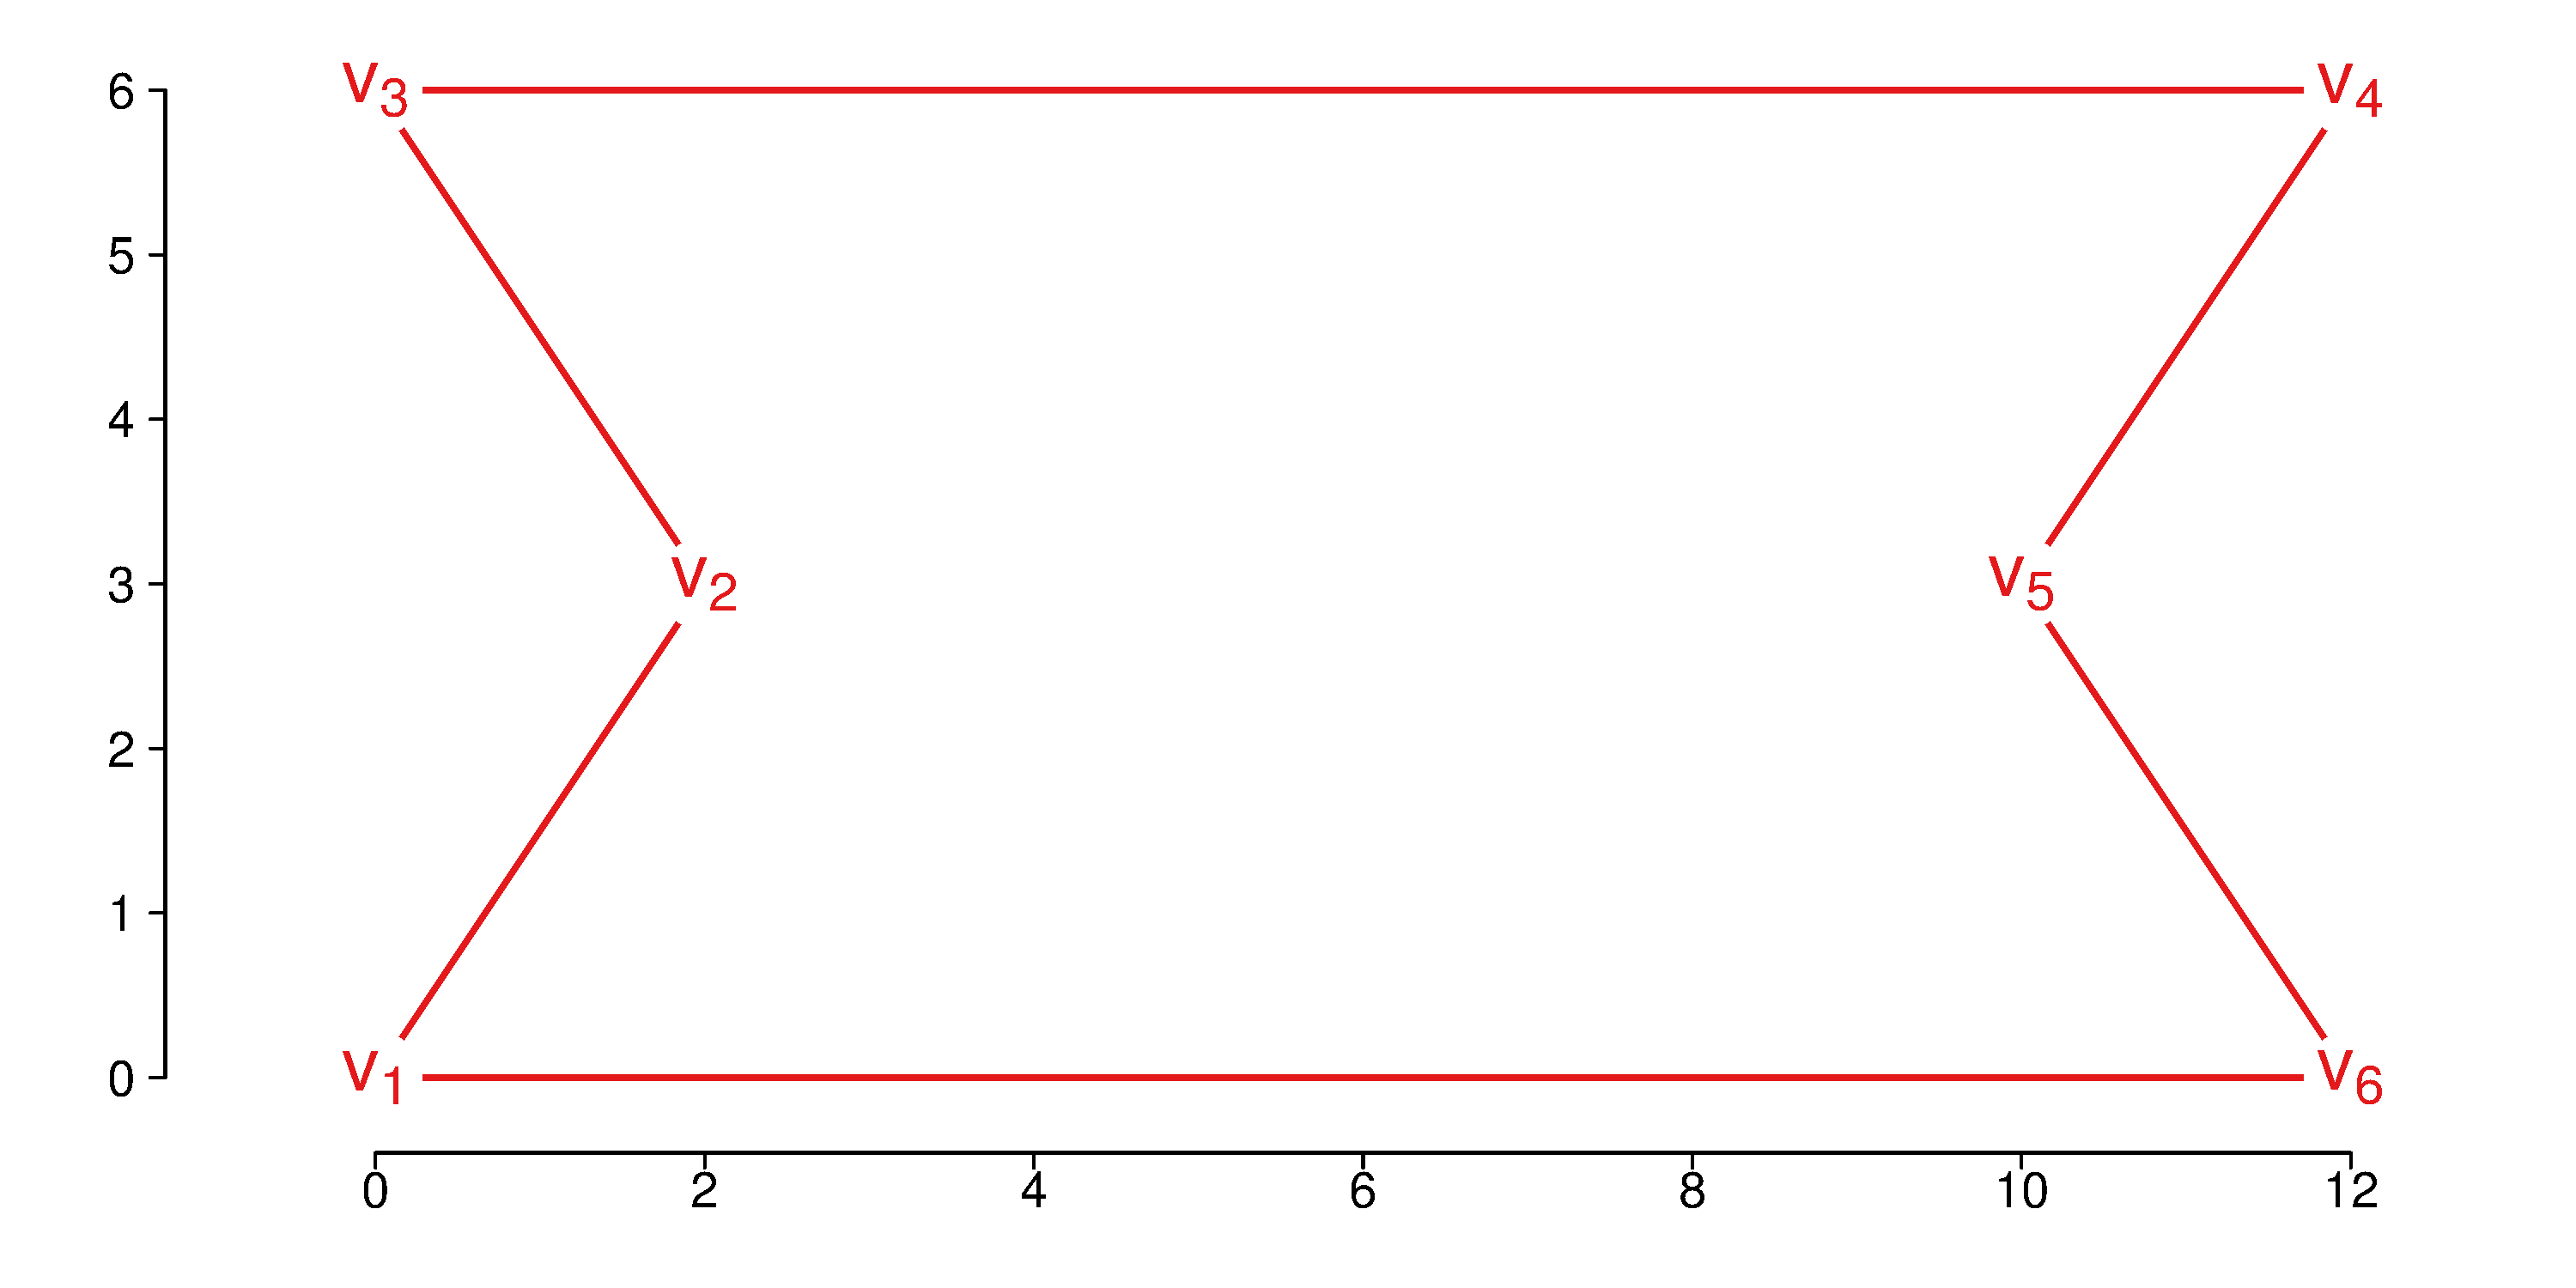
\includegraphics[height=1.7in]{rectangular-habitat-choose_grid04.png}
\end{tabular}
\caption{}
\end{subfigure}
\caption{The habitat is represented as a ring, i.e., a simple closed polygon without holes. (a) The ring should be \textit{closed}, i.e. the first vertex is also the last vertex. (b) The vertices should be listed \textit{counterclockwise}. (c) It is straightforward to specify habitats with complex irregular shape.}
\label{fig:habitat-examples}
\end{figure}
\clearpage}

\section{The population graph}

The population graph is a triangular grid contained entirely inside the habitat. The user specifies its density as a number of demes, `nDemes`, and EEMS constructs a grid with about the same number of demes that fills the habitat. This procedure is not necessarily optimal (i.e., it might not cover as much area as possible near the boundaries), and it might be helpful to iterate between refining the habitat specification and the number of demes `nDemes` to choose a satisfactory grid.

As an example, let's construct a graph for the African elephant dataset.

\afterpage{
\begin{figure}[!]

\begin{subfigure}[t]{0.45\textwidth}
\centering
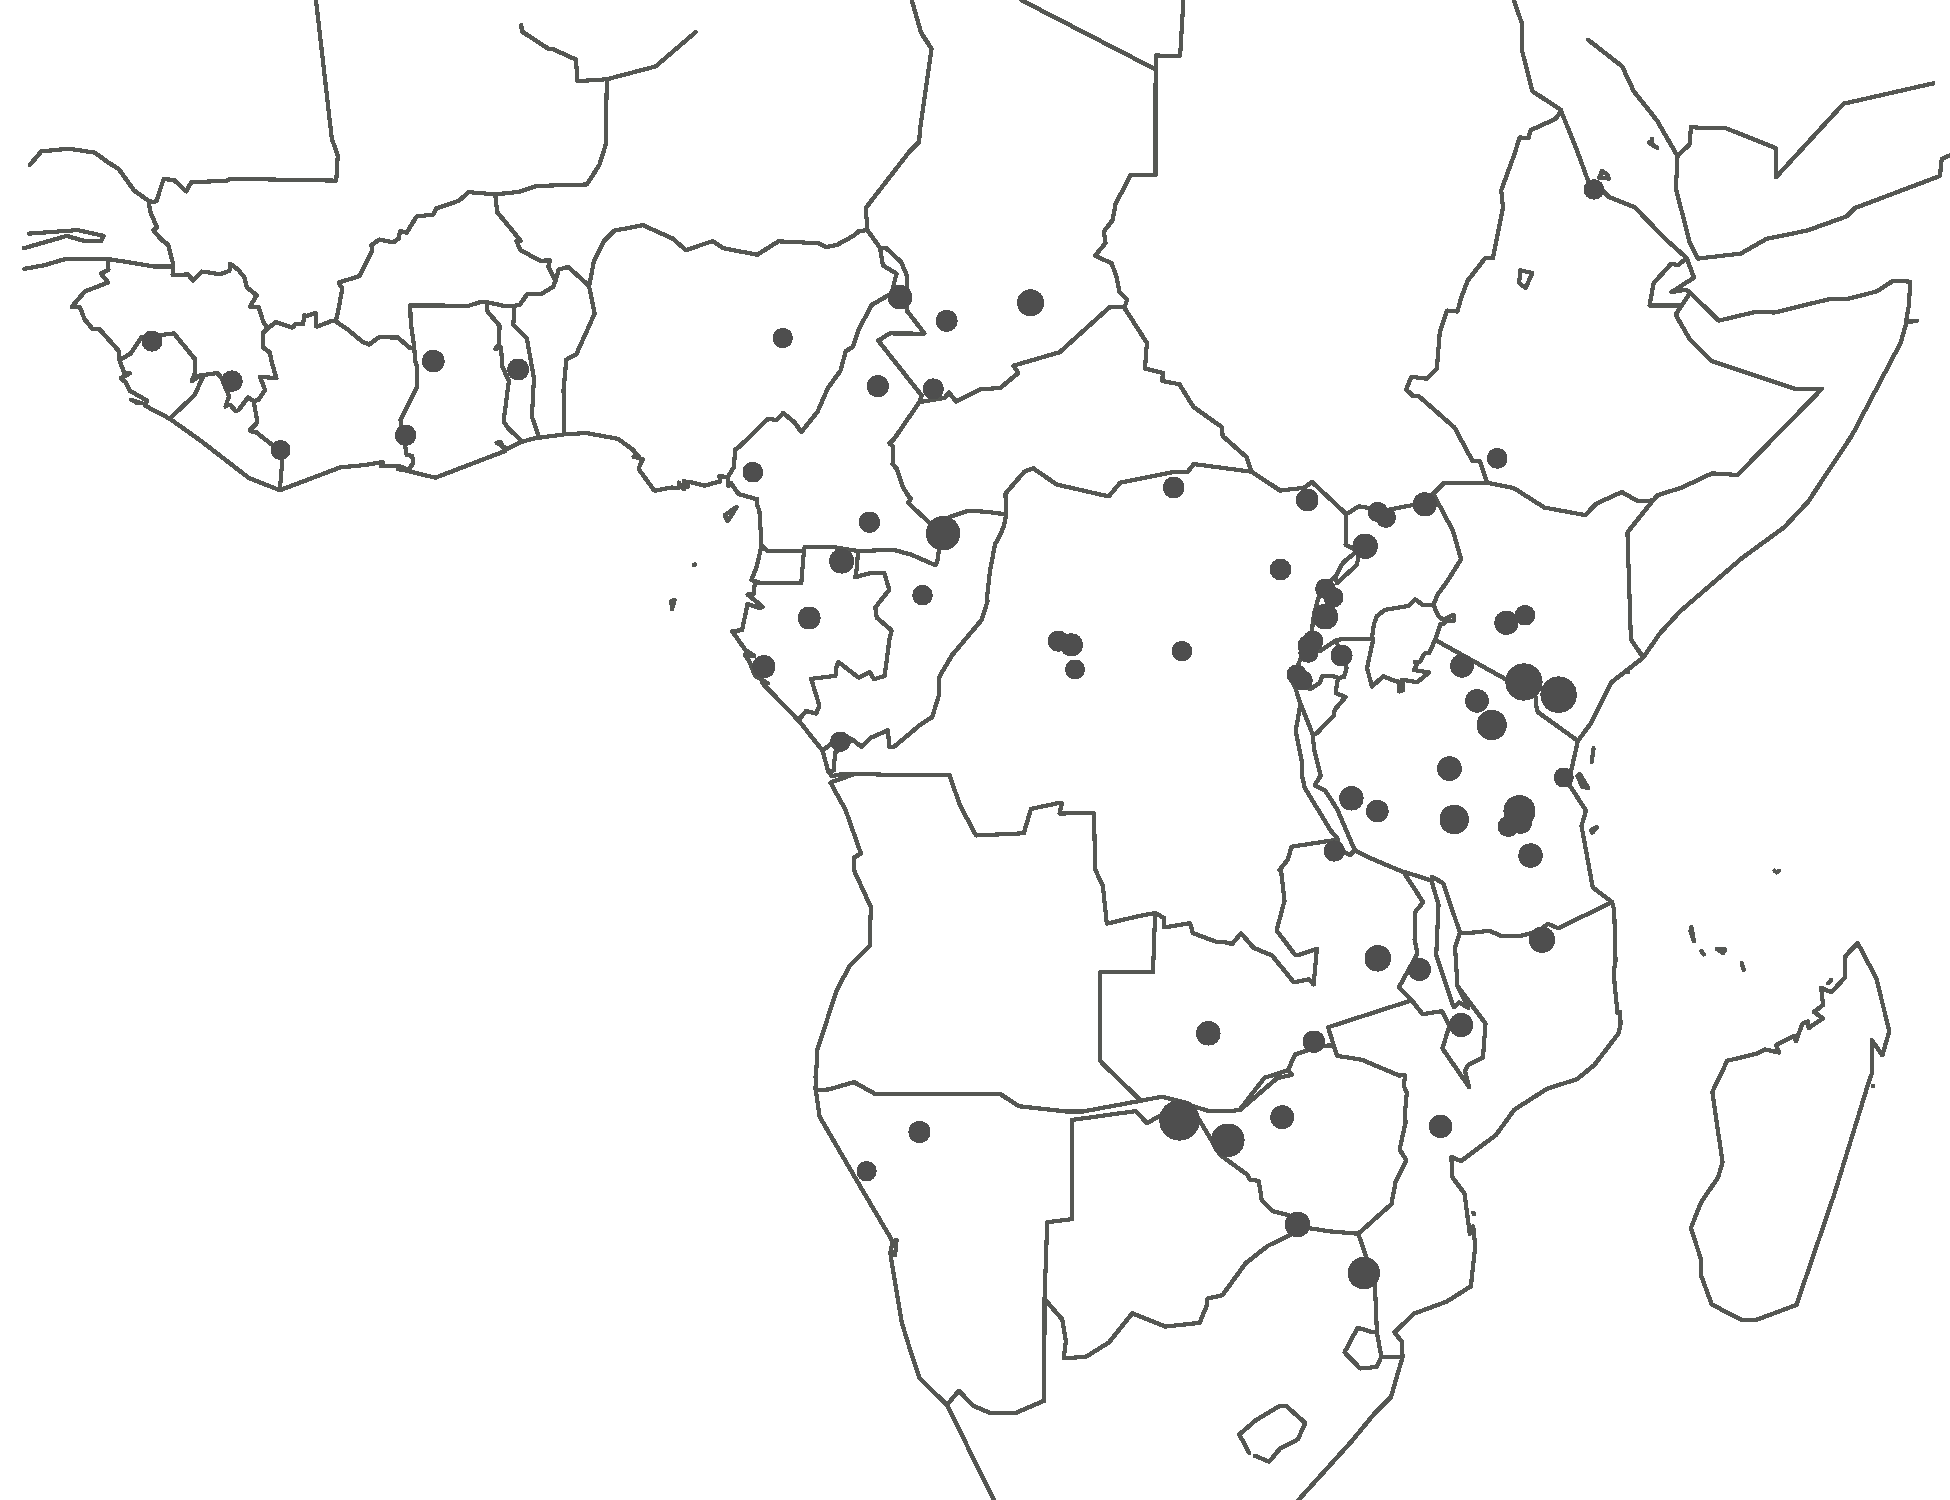
\includegraphics[height=2in]{V3b-nohyb-nIndiv1124-choose_grid01.png}
\caption{}
\end{subfigure}
\begin{subfigure}[t]{0.45\textwidth}
\centering
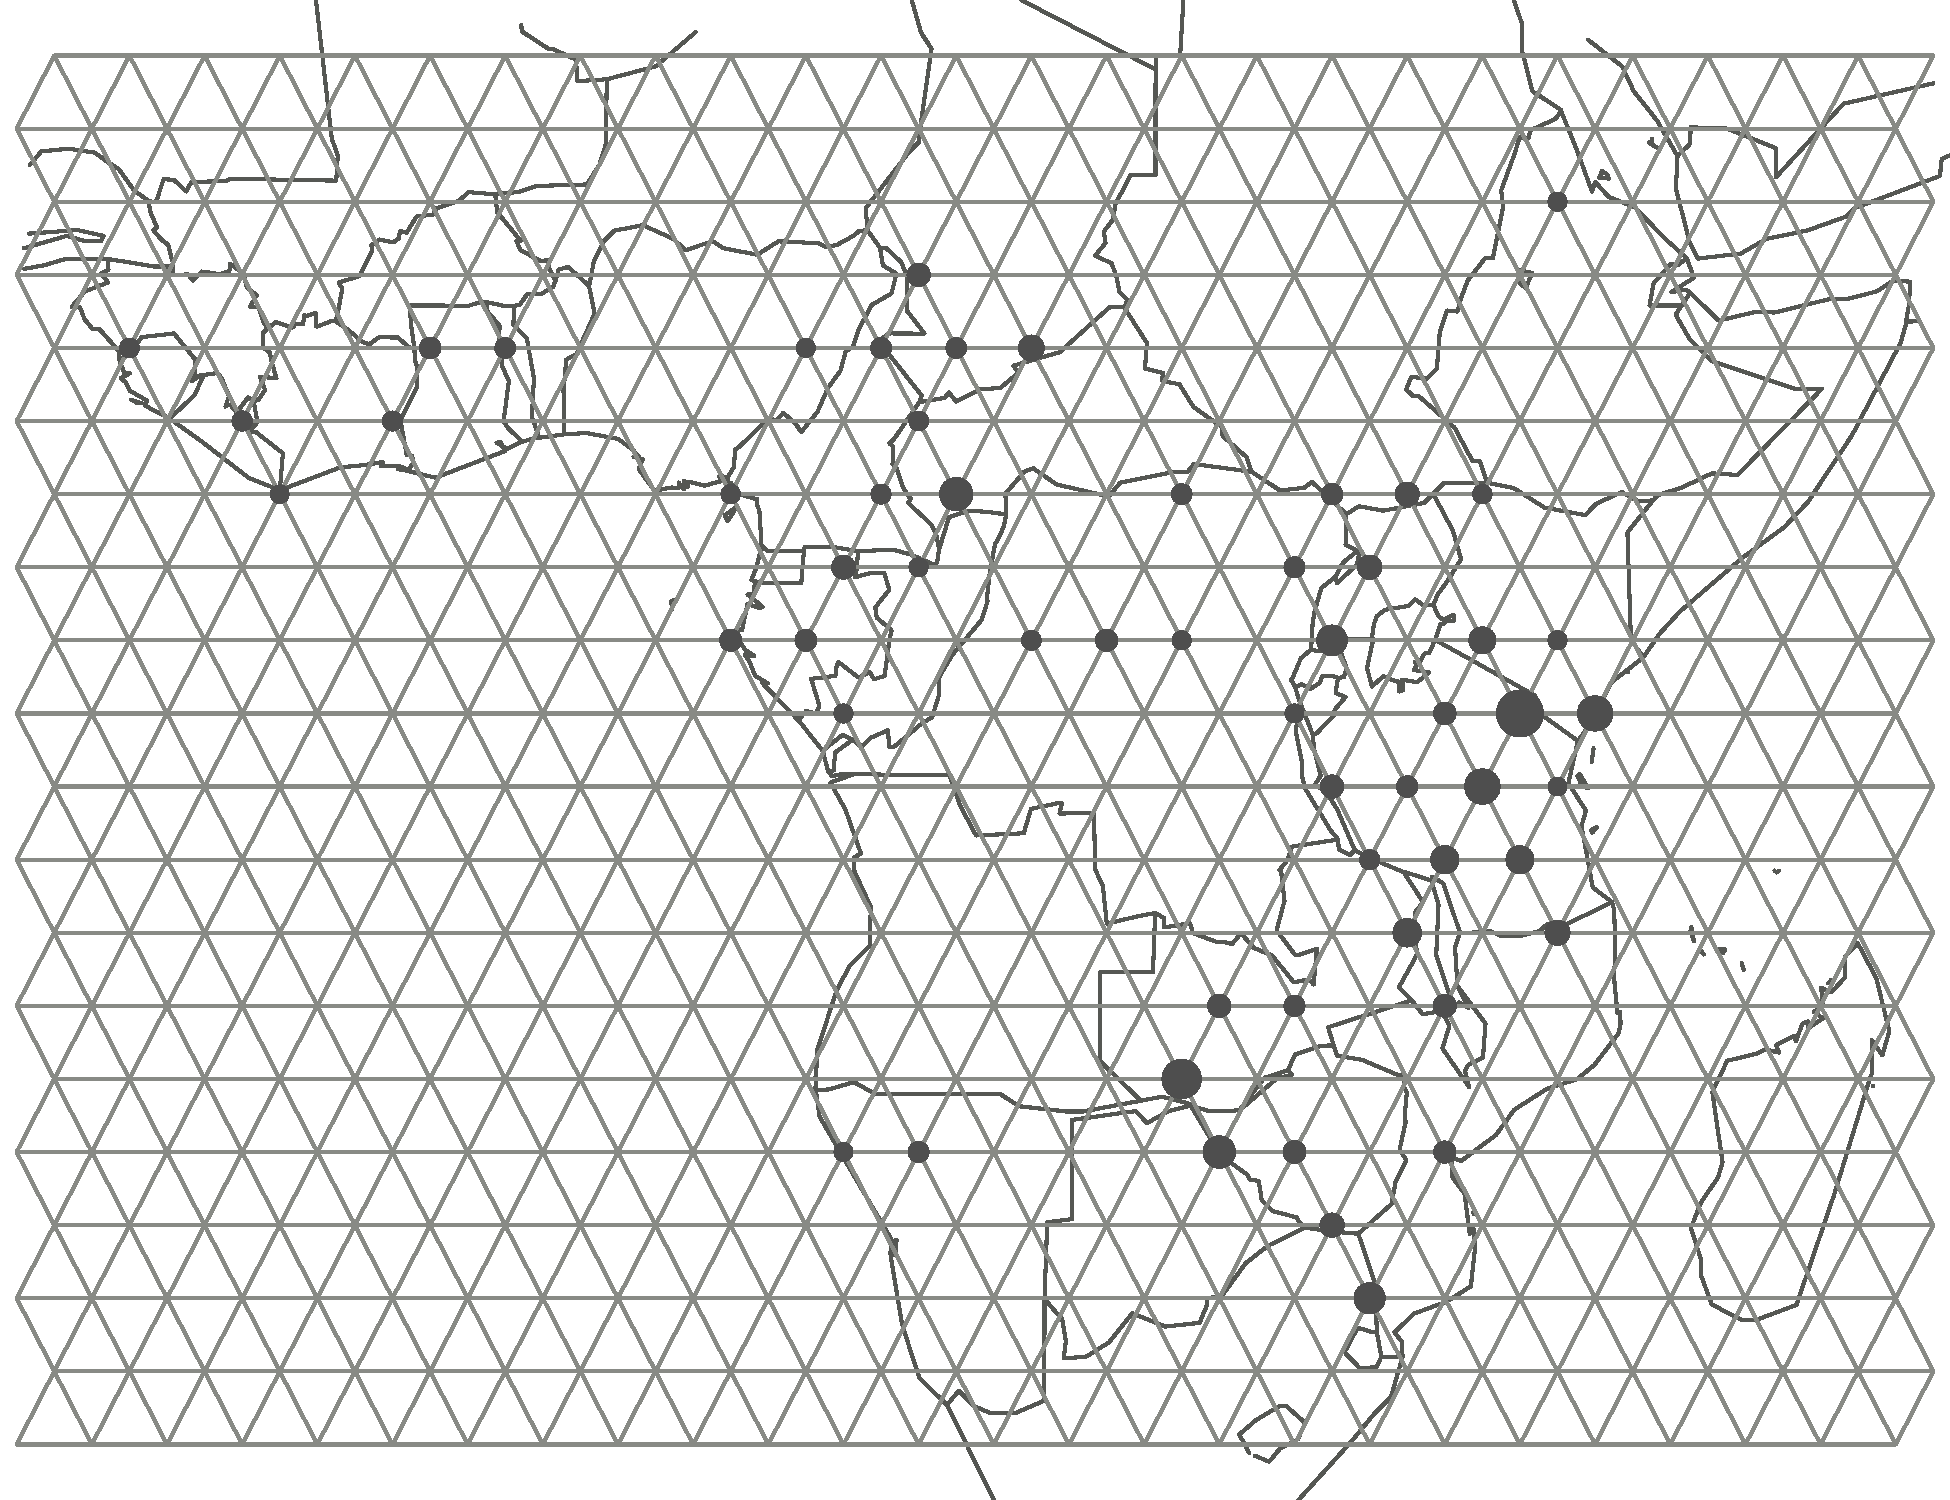
\includegraphics[height=2in]{V3b-nohyb-nIndiv1124-choose_grid02.png}
\caption{}
\end{subfigure}

\vspace{20pt}

\begin{subfigure}[t]{0.45\textwidth}
\centering
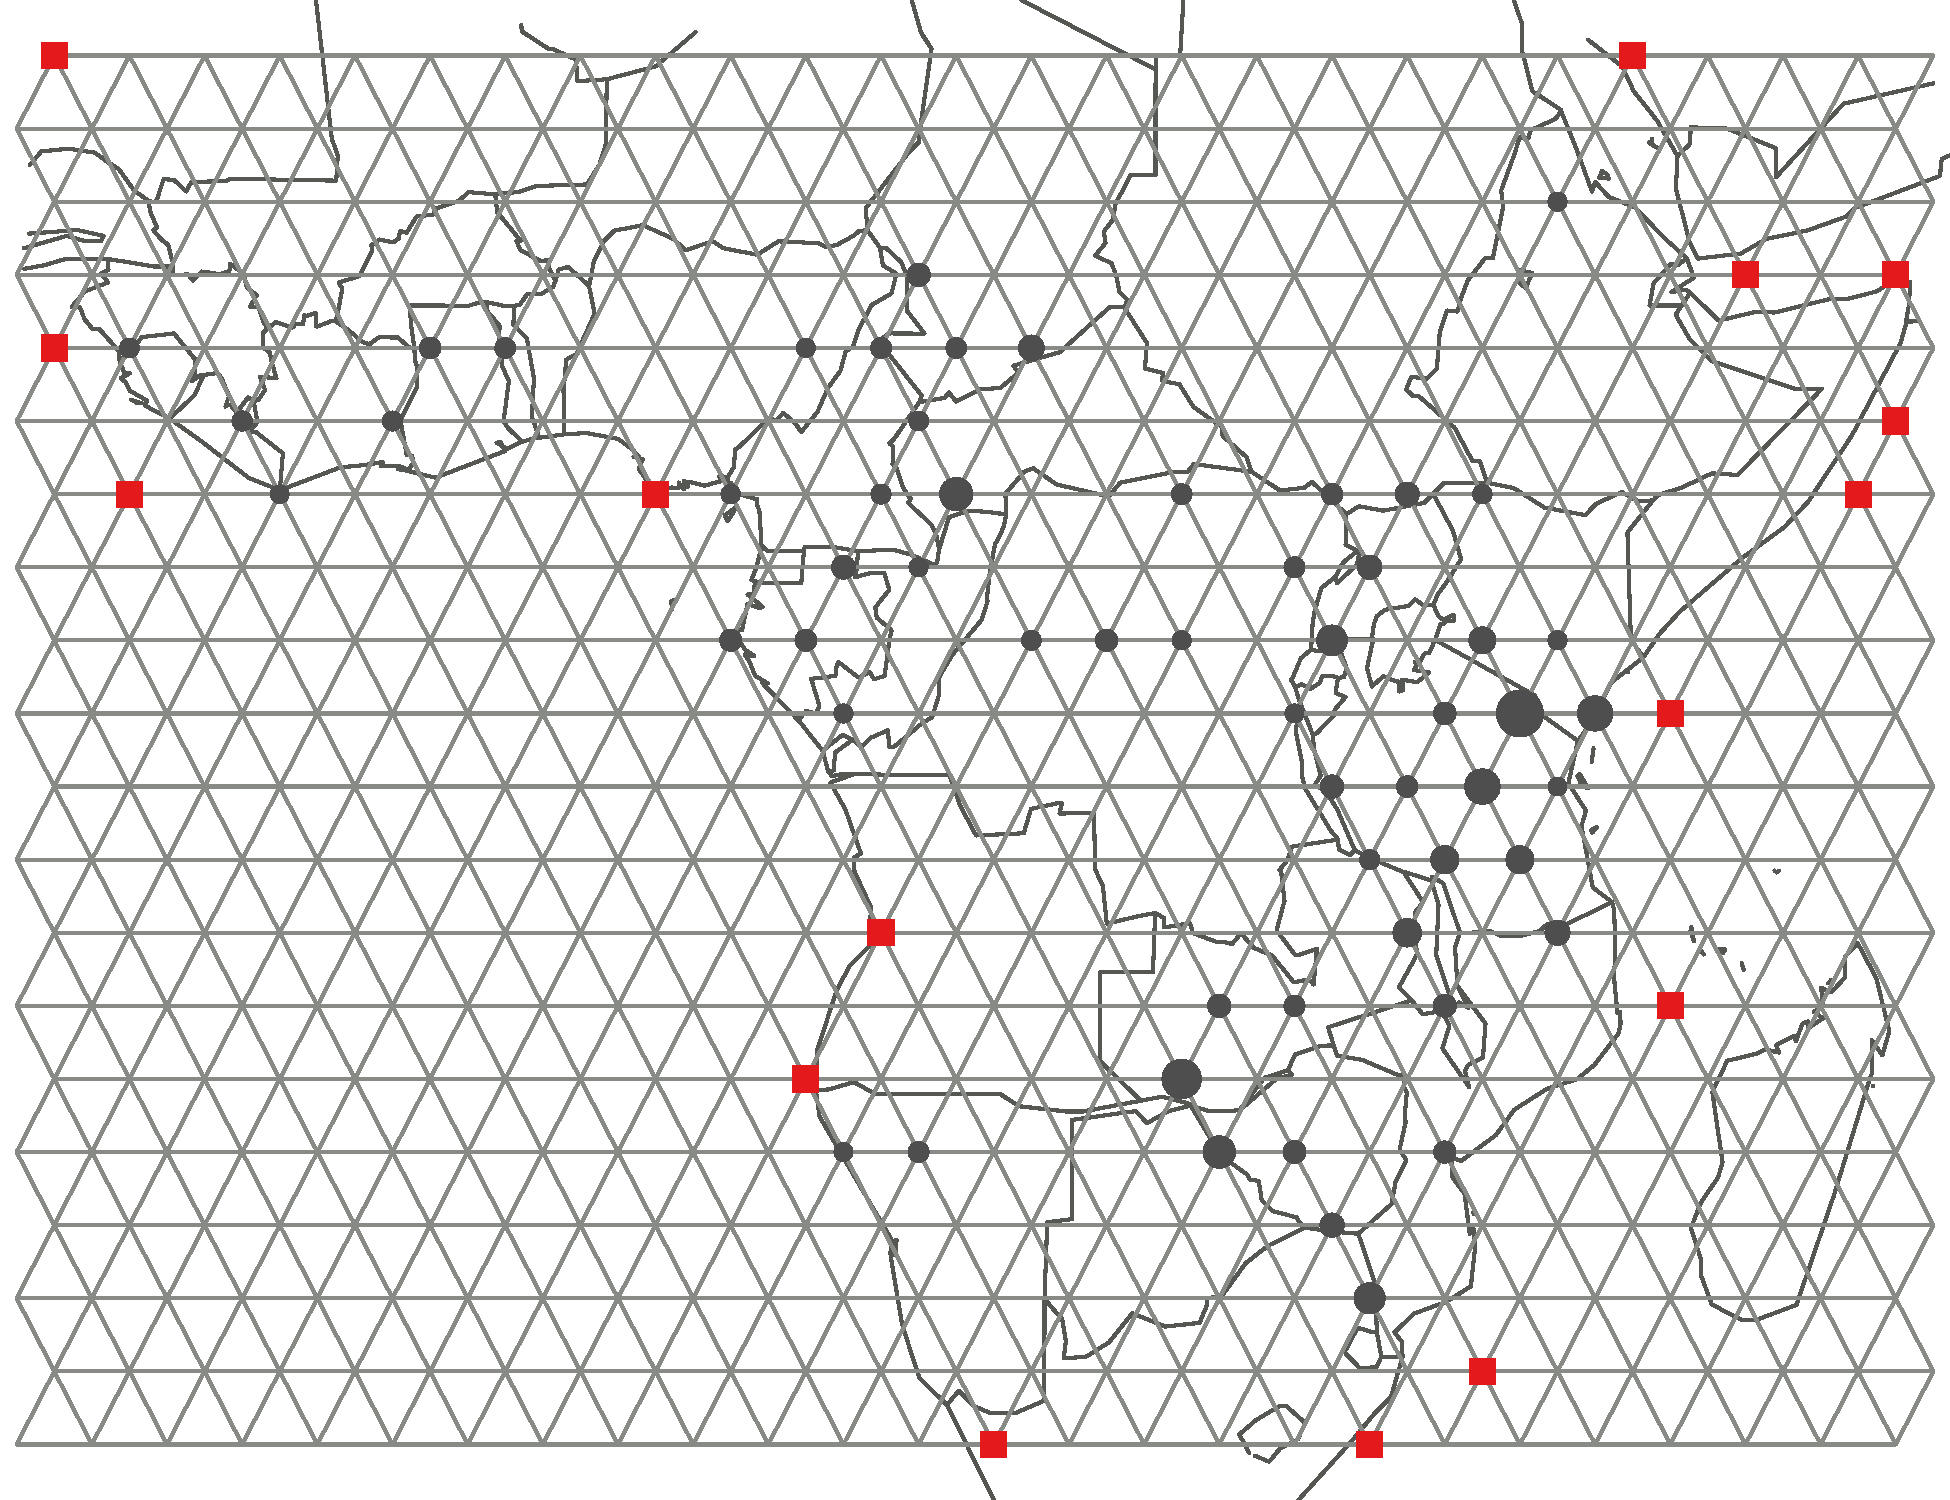
\includegraphics[height=2in]{V3b-nohyb-nIndiv1124-choose_grid03.png}
\caption{}
\end{subfigure}
\begin{subfigure}[t]{0.45\textwidth}
\centering
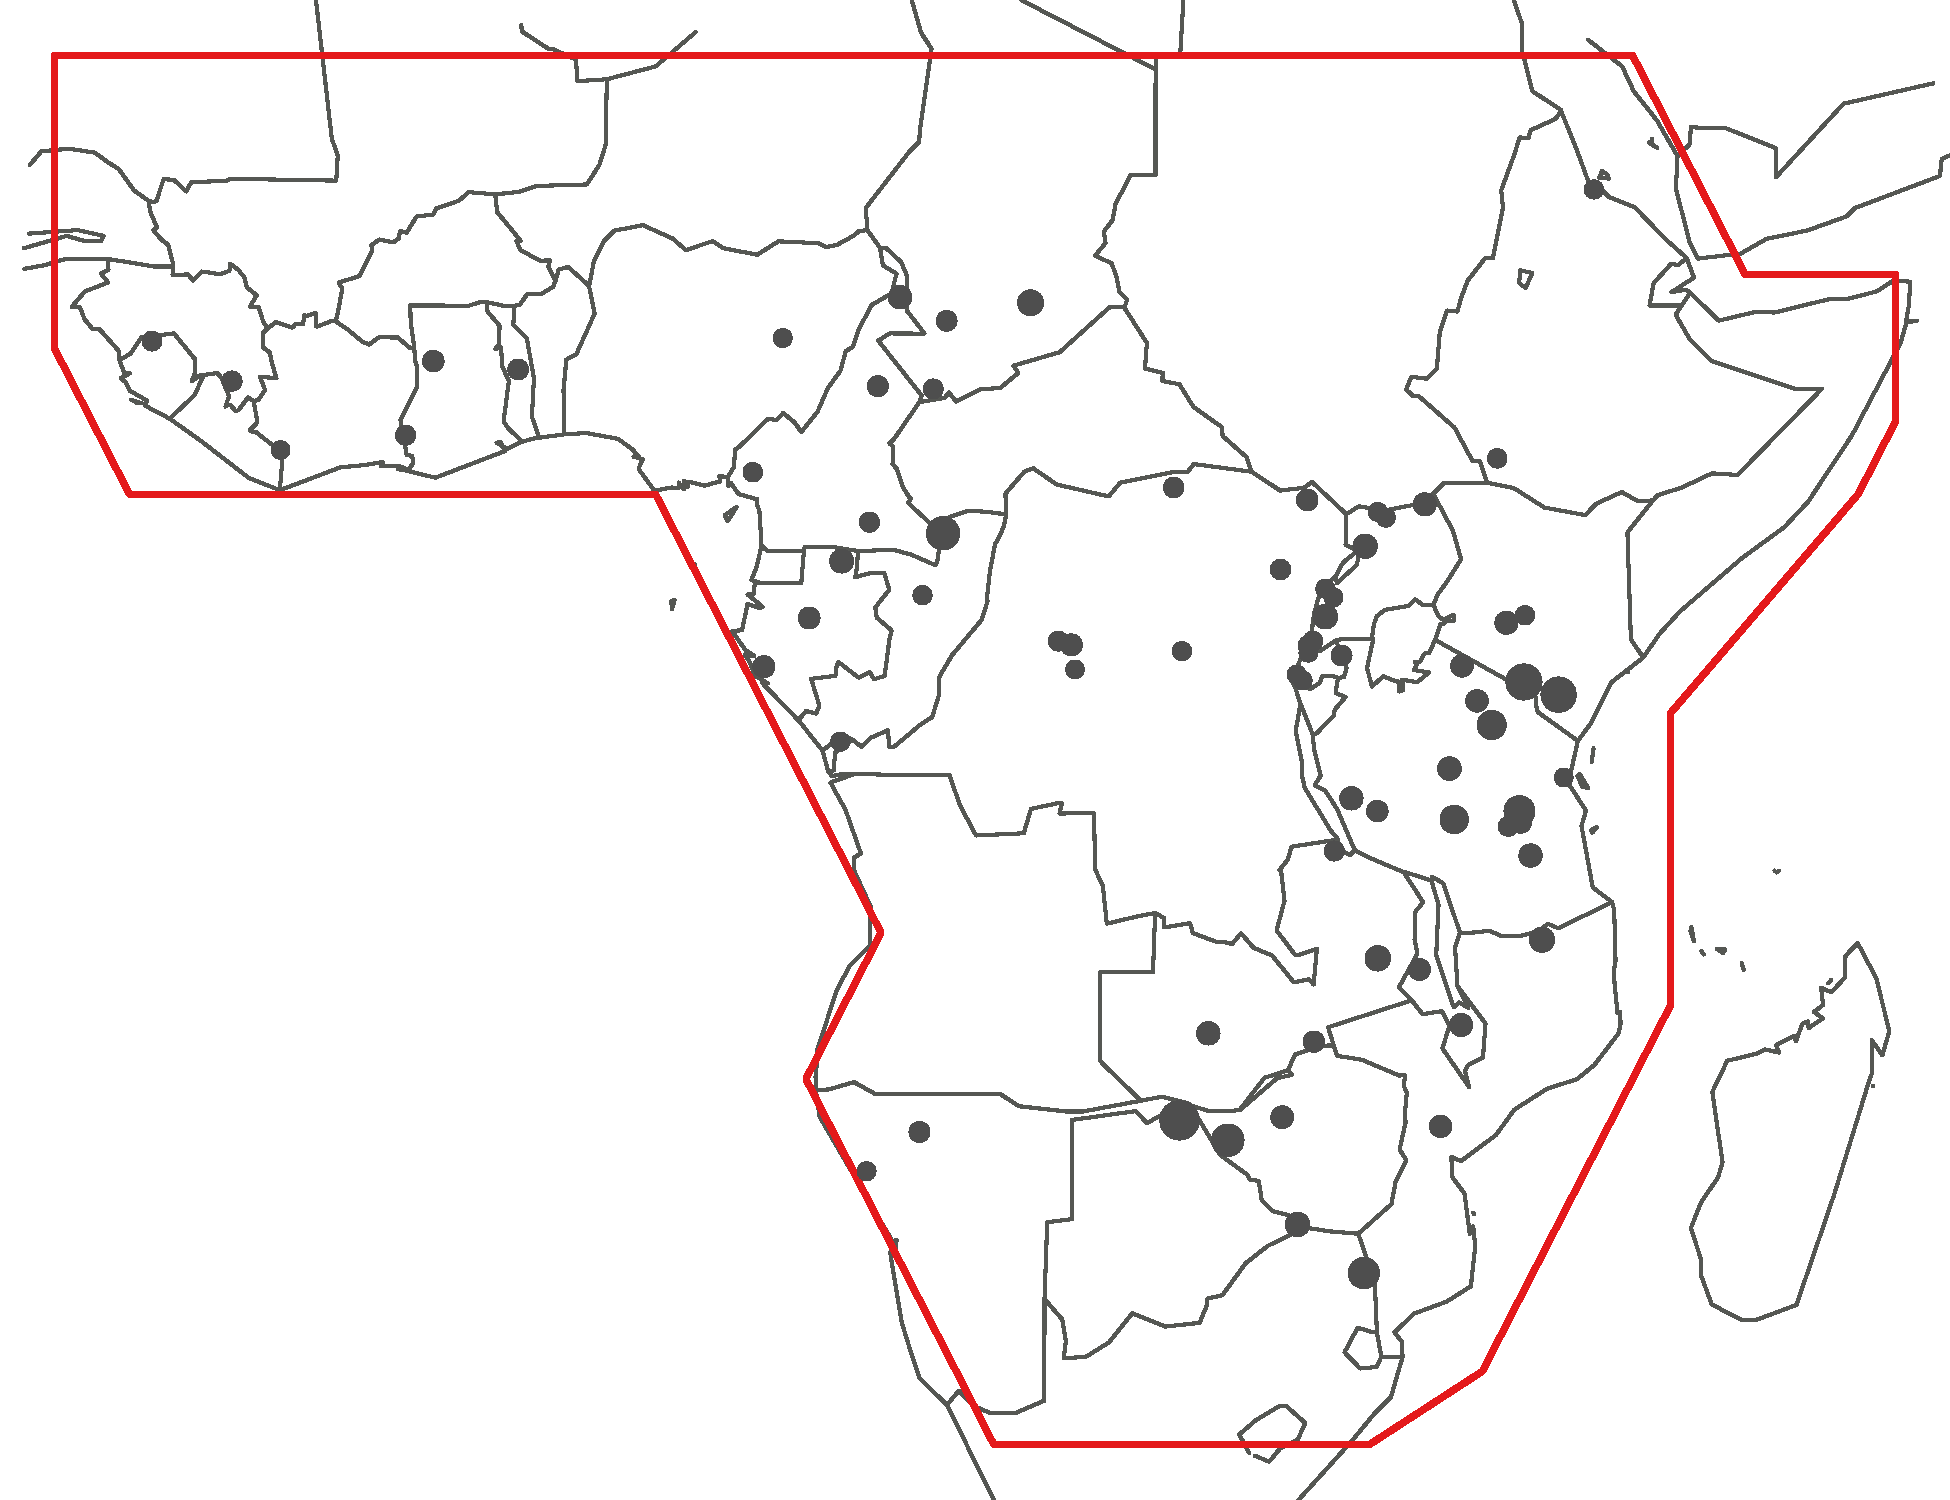
\includegraphics[height=2in]{V3b-nohyb-nIndiv1124-choose_grid04.png}
\caption{}
\end{subfigure}

\vspace{20pt}

\begin{subfigure}[t]{\textwidth}
\centering
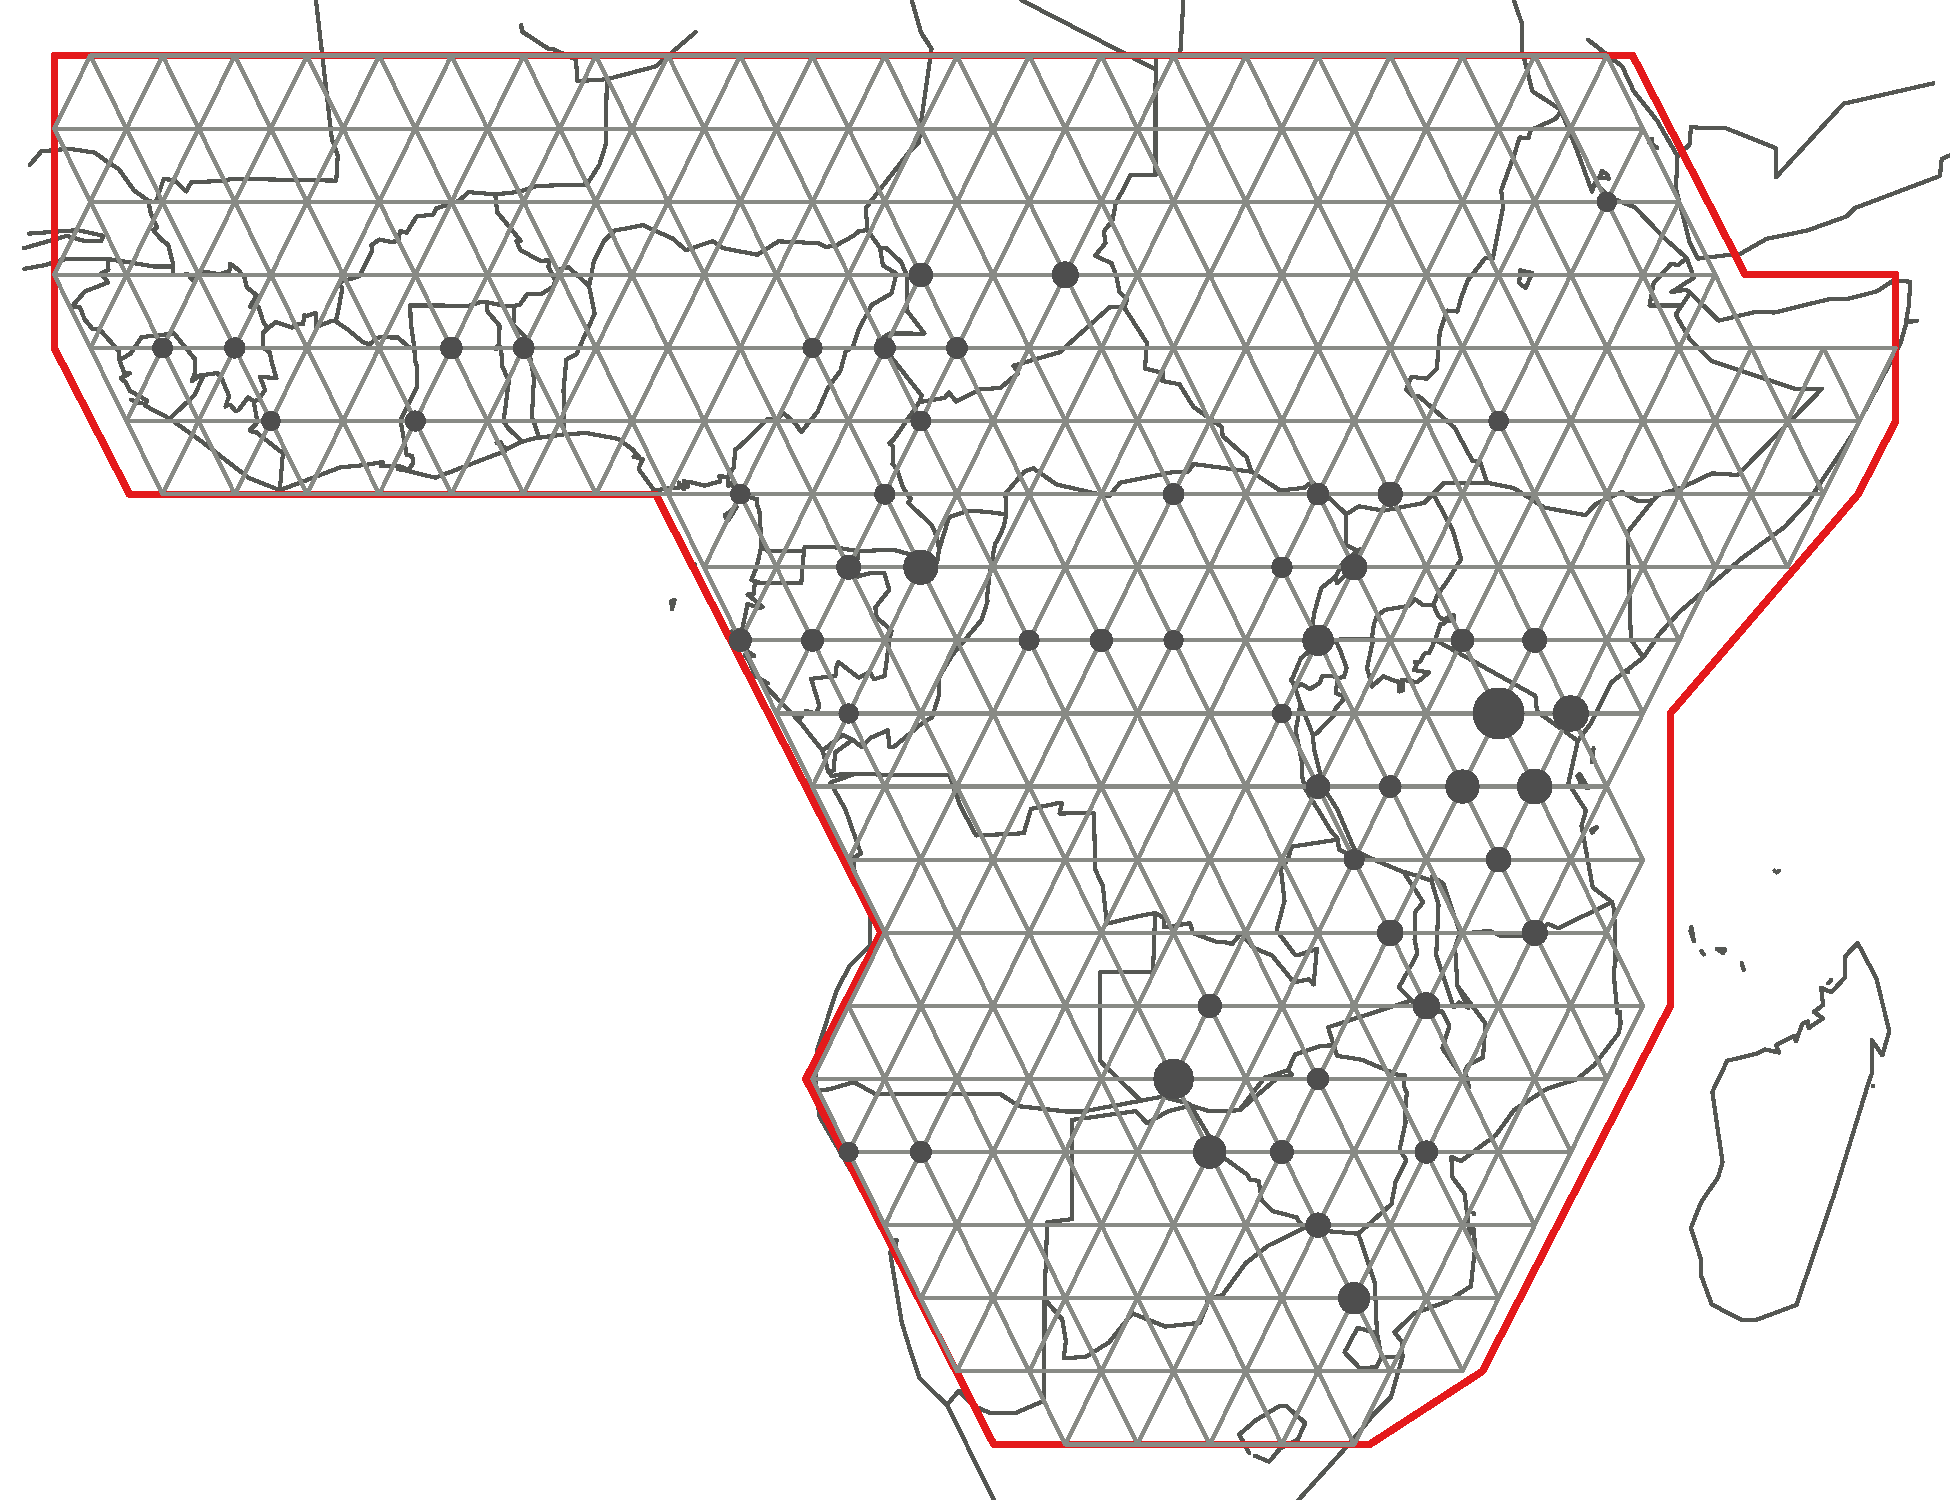
\includegraphics[height=2in]{V3b-nohyb-nIndiv1124-choose_grid05.png}
\caption{}
\end{subfigure}

\caption{This example shows how we can specify the habitat boundaries by first creating a rectangular grid and then picking a few vertices (in the rectangular grid) to outline the sampled habitat. (a) Samples are collected at known locations across a two-dimensional habitat. In this example, elephant samples are collected throughout Africa. (b) It is straightforward (using EEMS) to construct a triangular grid that spans a rectangular habitat because a rectangle is defined by only four vertices. However, we might want to exclude some regions from the ``habitat''; in the case of the African elephant, we might want to exclude the Atlantic and the Indian oceans. (c) We can choose a few vertices that approximately outline the habitat. (d) The resulting habitat has roughly the shape of Sub-Saharan Africa. (e) An irregularly shaped grid is generated automatically by EEMS given the irregular habitat outline (in red) and the deme density.}
\end{figure}
\clearpage}

\newpage
\section{Input parameters}

There are a number of program parameters that can be set by the user. First, there are several parameters that have to be specified (there are no default values for those):
\begin{itemize}
  \item `datapath`: path to the input data. For SNP data, EEMS expects three files: a matrix of average pairwise differences, \textit{datapath}.diffs; a list of sample coordinates, \textit{datapath}.coord; a list of habitat boundary points, \textit{datapath}.outer. For microsatellite data, EEMS also expects three files: a matrix of allele copies, \textit{datapath}.sites; a list of sample coordinates, \textit{datapath}.coord; a list of habitat boundary points, \textit{datapath}.outer.
  \item `mcmcpath`: path to the output directory. EEMS creates this directory and saves all results there. (There is an accompanying R script which parses the output files and generates several figures that represent the EEMS results.)
  \item `nIndiv` and `nSites`: number of samples and number of markers.
  \item `numMCMCIter`, `numBurnIter`, `numThinIter`: number of MCMC iterations, number of burn-in iterations to discard at the start, and number of iterations to thin between two writing steps.
  \item `nDemes`: the (approximate) number of demes in the population graph. If the habitat is irregular, the actual number of demes in the grid might not be exactly equal to the specified number of demes.
\end{itemize}

Additionally, there are several extra parameters that can be specified optionally (they have default values but modifying those values could improve convergence).

\begin{itemize}
\item Variances for the proposal distributions of migration parameters:
\begin{itemize}
  \item `mEffctProposalS2`: proposal variance for the migration cell effects, $e_1,\ldots,e_{C_m}$
  \item `mSeedsProposalS2`: proposal variance for the migration cell locations, $s_1,\ldots,s_{C_m}$
  \item `mrateMuProposalS2`: proposal variance for the overall migration rate $\mu$ (on the $\log_{10}$ scale)
\end{itemize}
\item Variances for the proposal distributions of diversity parameters:
\begin{itemize}
  \item `qEffctProposalS2`: proposal variance for the diversity cell effects, $f_1,\ldots,f_{C_q}$
  \item `qSeedsProposalS2`: proposal variance for the diversity cell locations, $t_1,\ldots,t_{C_q}$
\end{itemize}
\item Hyperparameters:
\begin{itemize}
  \item `mrateShape,mrateScale`: (inverse gamma) hyperparameters for the variance $\omega_m^2$ of the migration effects
  \item `qrateShape,qrateScale`: (inverse gamma) hyperparameters for the variance $\omega_q^2$ of the diversity effects
  \item `s2locShape,s2locShape`: (inverse gamma) hyperparameters for the scale parameters $\sigma_1^2,\ldots,\sigma_p^2$
  \item `negBiSize`: number of failures for the Negative-Binomial prior on the number of Voronoi tiles
  \item `negBiProb`: success probability for the Negative-Binomial prior on the number of Voronoi tiles
\end{itemize}
\end{itemize}

\newpage
\section{Running EEMS -- an example}

This example shows how to run EEMS on a small simulated dataset (one of the ``barrier to migration'' datasets used for Figure 2 in the EEMS paper.)

First, create three input parameter files. All parameters are the same, except for the output directory `mcmcpath`.

\bigskip

\noindent params-simno1.ini:
\begin{verbatim}
datapath = ./data/barrier-schemeX-nIndiv300-nSites3000
mcmcpath = ./data/barrier-schemeX-nIndiv300-nSites3000-EEMS-nDemes153-simno1
nIndiv = 300
nSites = 3000
nDemes = 200
diploid = false
numMCMCIter = 20000
numBurnIter = 10000
numThinIter = 99
\end{verbatim}

\noindent params-simno2.ini:
\begin{verbatim}
datapath = ./data/barrier-schemeX-nIndiv300-nSites3000
mcmcpath = ./data/barrier-schemeX-nIndiv300-nSites3000-EEMS-nDemes153-simno2
nIndiv = 300
nSites = 3000
nDemes = 200
diploid = false
numMCMCIter = 20000
numBurnIter = 10000
numThinIter = 99
\end{verbatim}

\noindent params-simno3.ini:
\begin{verbatim}
datapath = ./data/barrier-schemeX-nIndiv300-nSites3000
mcmcpath = ./data/barrier-schemeX-nIndiv300-nSites3000-EEMS-nDemes153-simno3
nIndiv = 300
nSites = 3000
nDemes = 200
diploid = false
numMCMCIter = 20000
numBurnIter = 10000
numThinIter = 99
\end{verbatim}

Then run EEMS (on the command line) on the simulated dataset, with three different random seeds. (The argument {\tt --seed} is optional; if not specified, the seed is randomly assigned.)

\begin{verbatim}
./runeems_snps --params params-simno1.ini --seed 123
./runeems_snps --params params-simno2.ini --seed 456
./runeems_snps --params params-simno3.ini --seed 789
\end{verbatim}

Finally, plot the results (in an R console).

\begin{verbatim}
source('default.eems.plots.R')

mcmcpath <- 
      paste('barrier-schemeX-nIndiv300-nSites3000-EEMS-nDemes153-simno',1:3,sep='')
plotpath <- 'barrier-schemeX-nIndiv300-nSites3000-EEMS-nDemes153-simno1_3'

## mcmcpath is a list of three output directories; the results are averaged                                                                                
eemsplots(mcmcpath,plotpath,add.map=FALSE)
\end{verbatim}

\afterpage{
\begin{figure}[!]

\begin{subfigure}[t]{\textwidth}
\centering
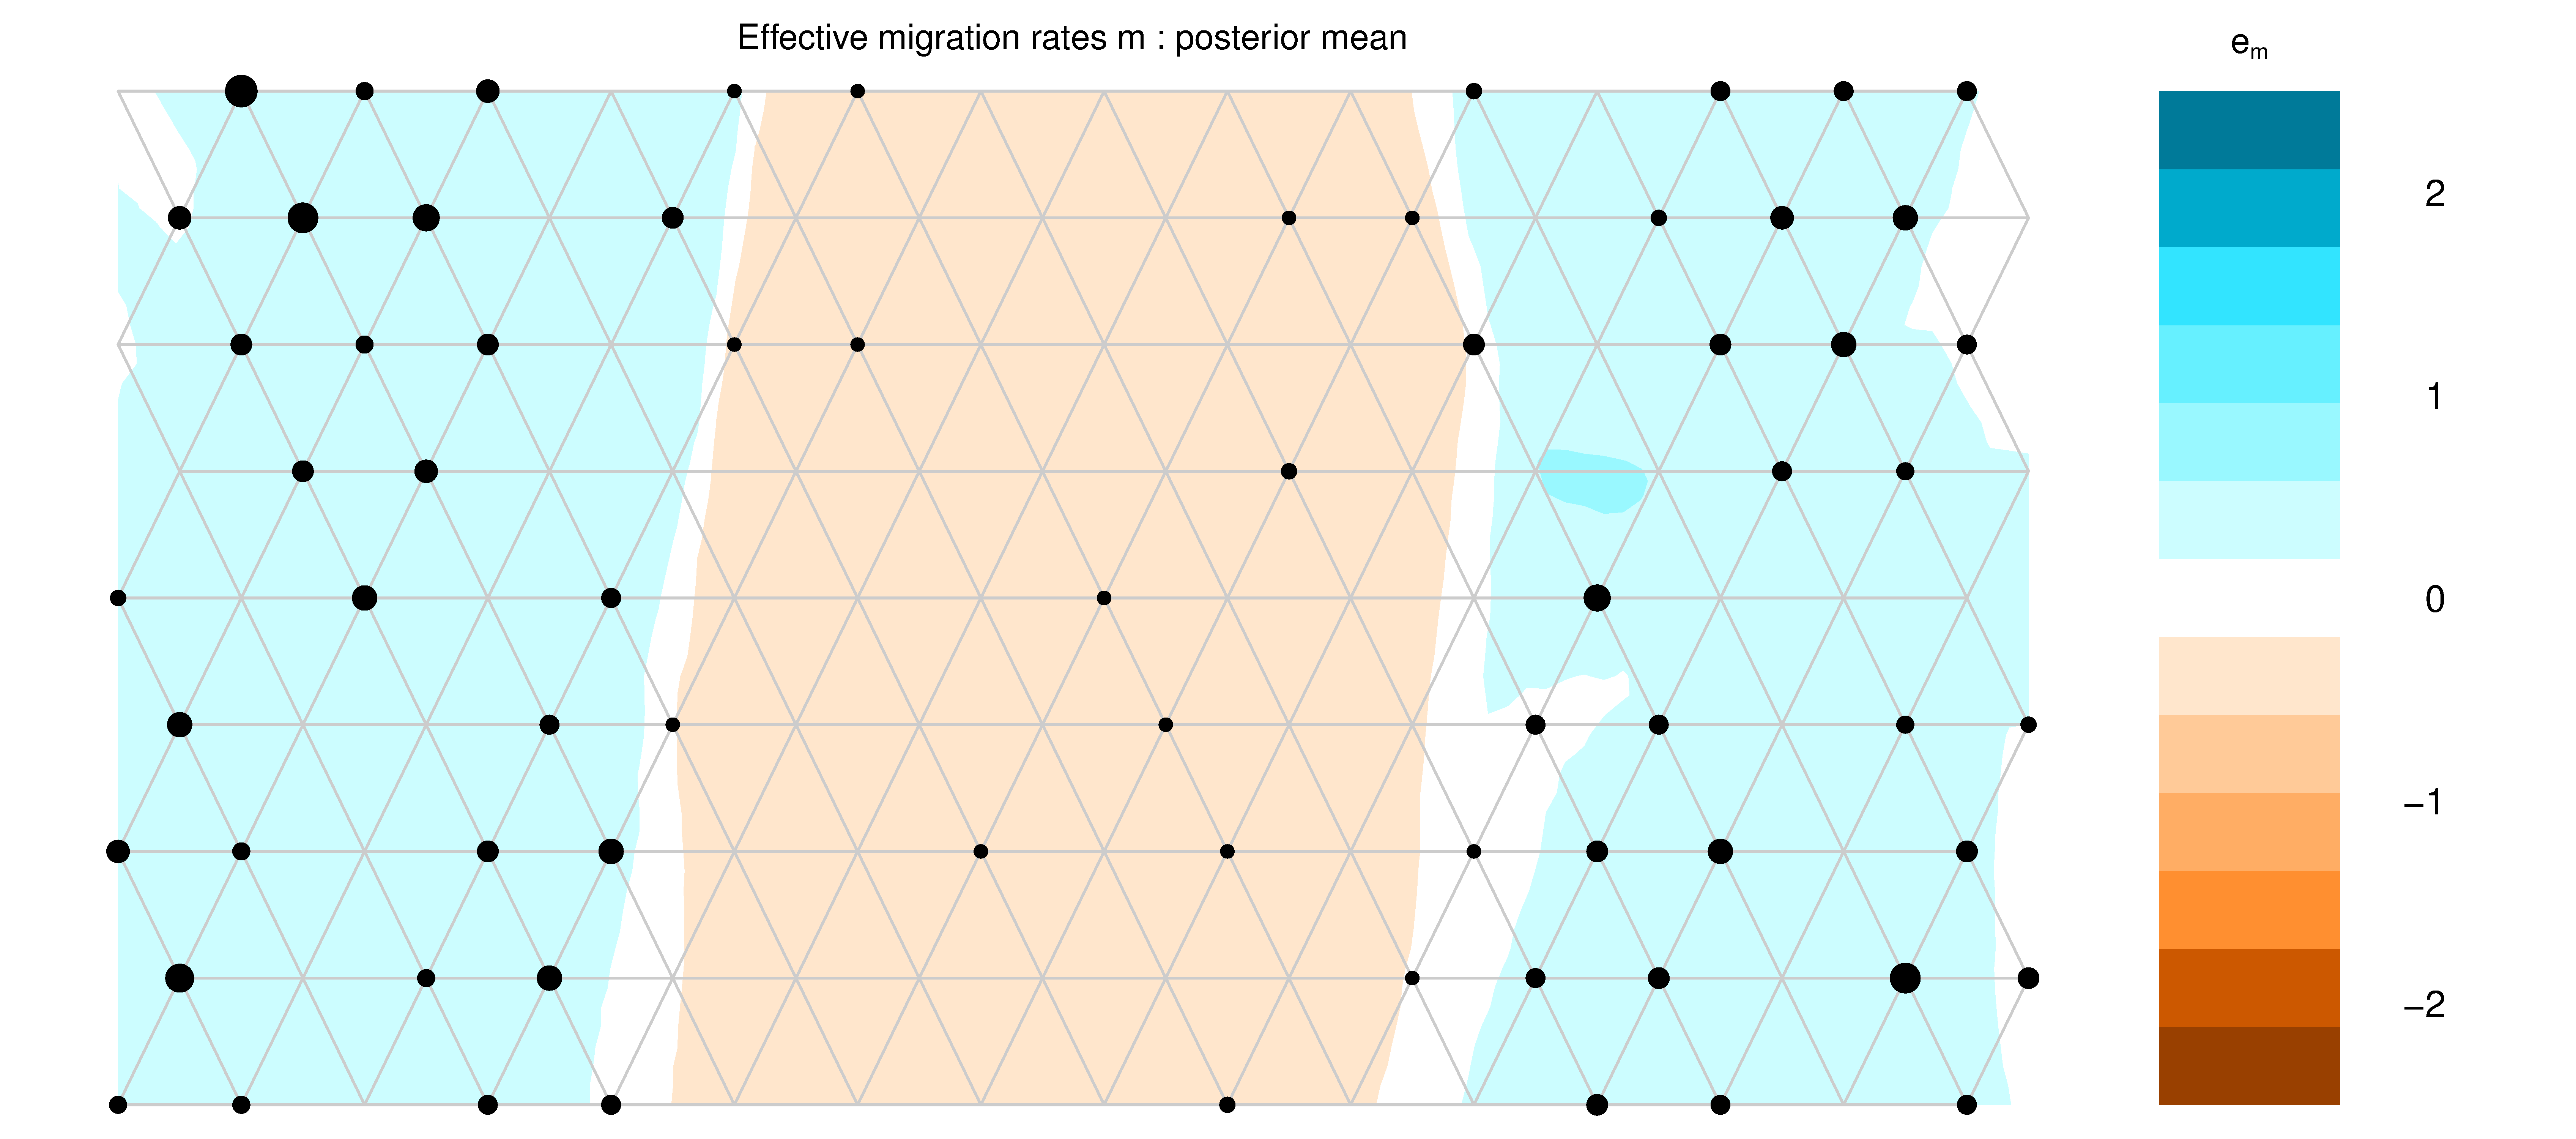
\includegraphics[height=2.4in]{barrier-schemeX-nIndiv300-nSites3000-EEMS-nDemes153-simno1_3-mrates01.png}
\caption{}
\end{subfigure}

\vspace{20pt}

\begin{subfigure}[t]{\textwidth}
\centering
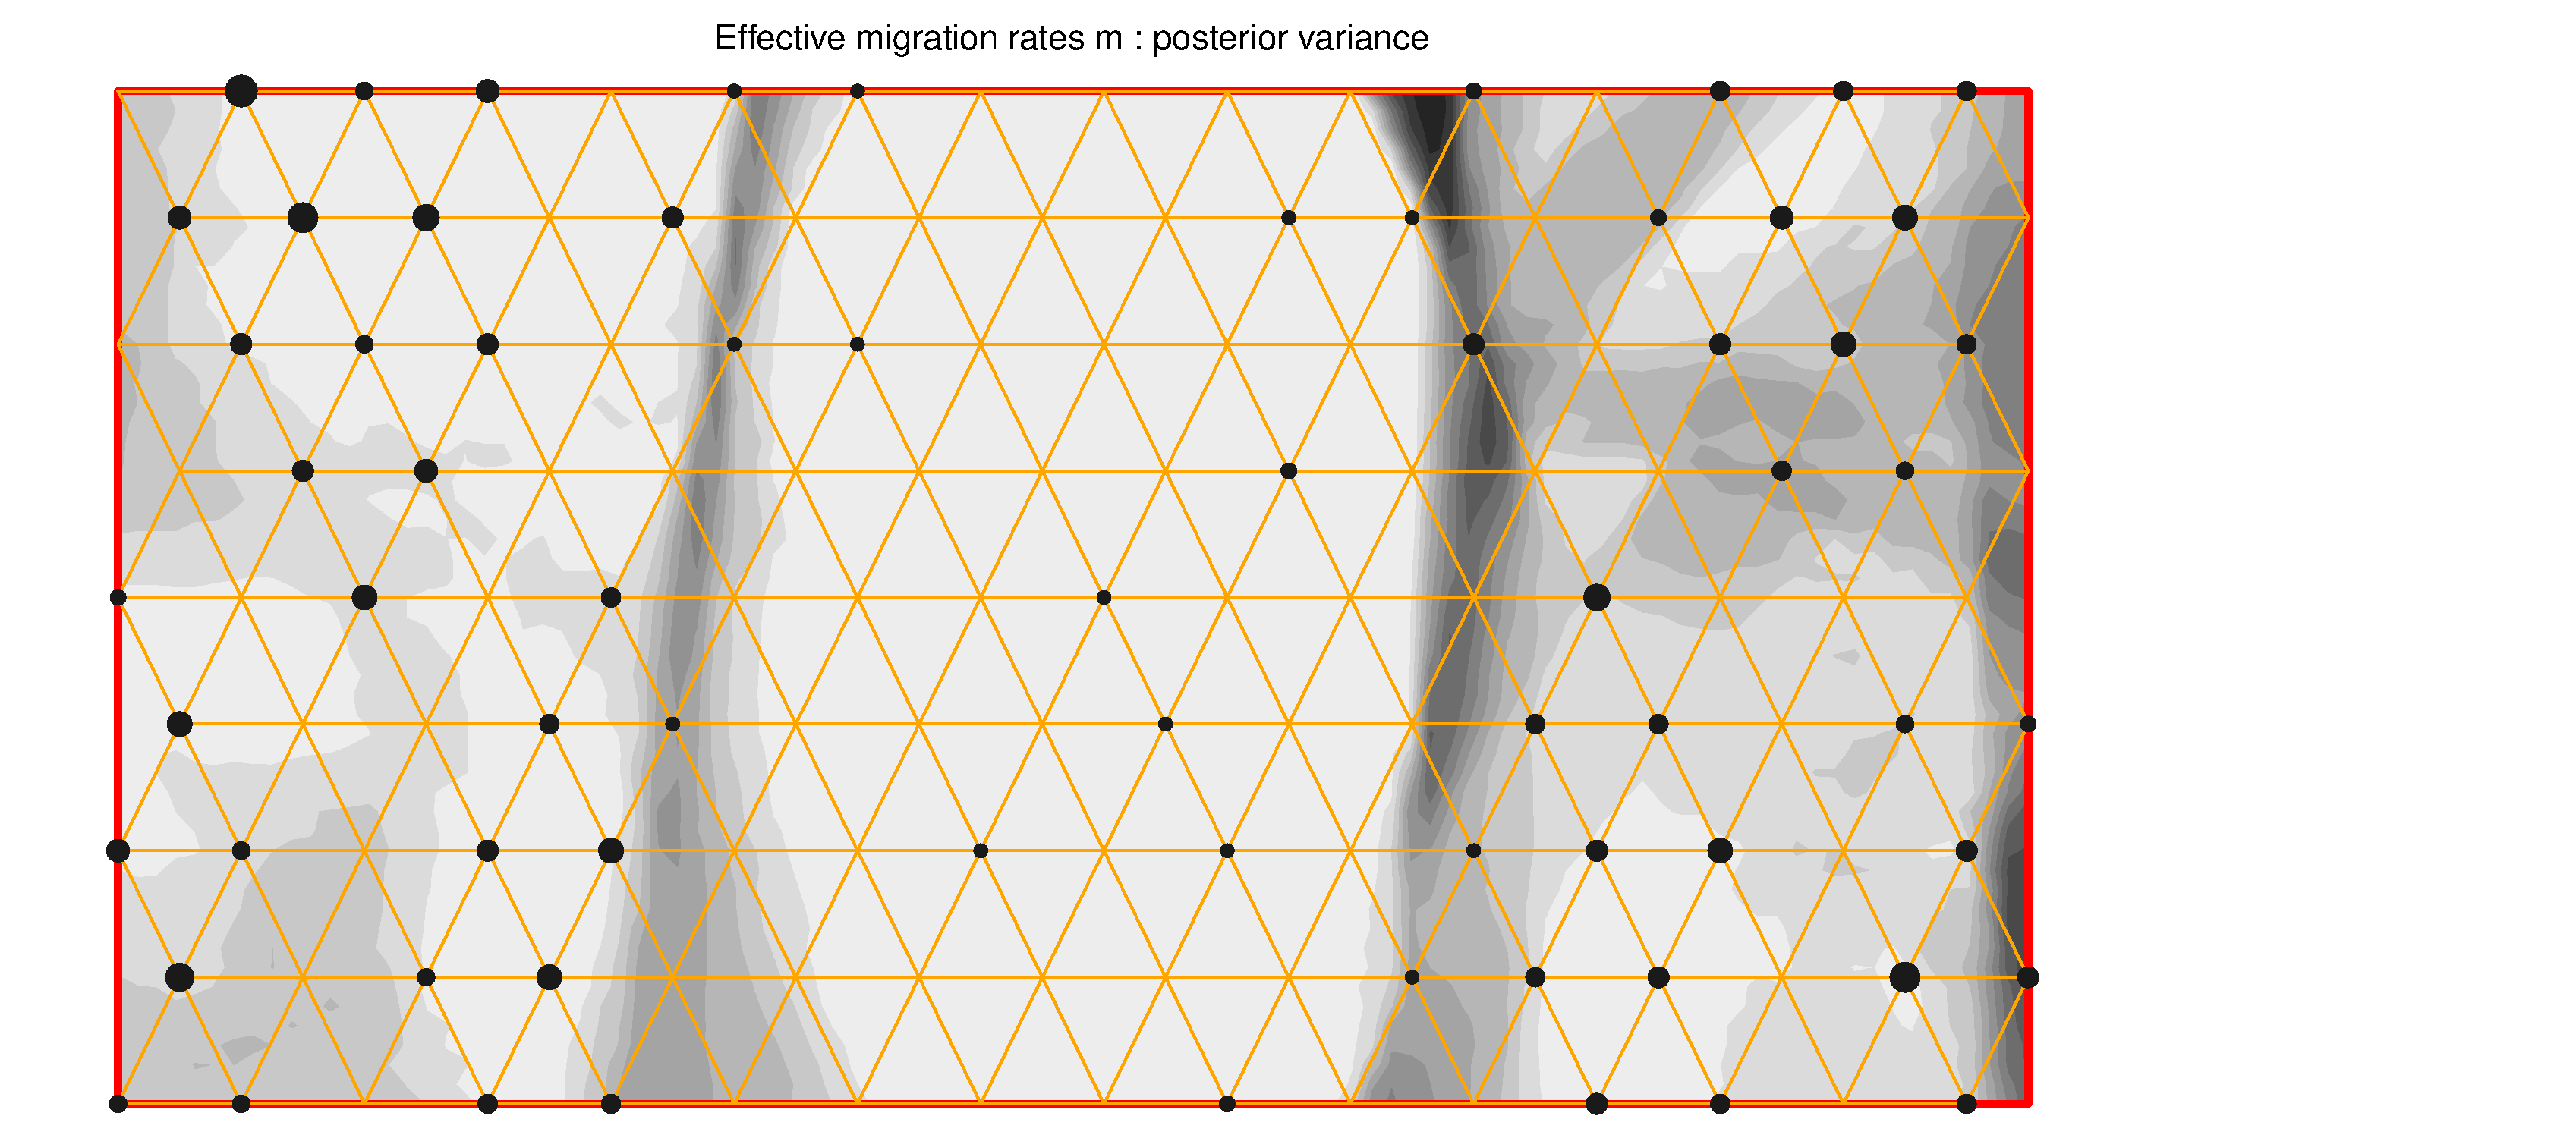
\includegraphics[height=2.4in]{barrier-schemeX-nIndiv300-nSites3000-EEMS-nDemes153-simno1_3-mrates02.png}
\caption{}
\end{subfigure}

\caption{EEMS analysis of a ``barrier to migration`` simulation. (a) Estimated effective migration surface. (b) (Relative) Variance of the posterior mean migration surface. The migration rates in some regions are estimated with more certainty than in other regions, and this can be illustrated by plotting the variance in the estimated effective migration surface. In this black-and-white contour plot, black means high variance and white means low variance; the posterior variance is rescaled to range from 0 to 1 as $(v_{xy}-v_{min})/(v_{max}-v_{min})$, where $v_{xy}$ is the variance at location $(x,y)$ and $v_{min},v_{max}$ are the lowest and the highest variance across all locations.}
\end{figure}
\clearpage}

\afterpage{
\begin{figure}[!]

\begin{subfigure}[t]{\textwidth}
\centering
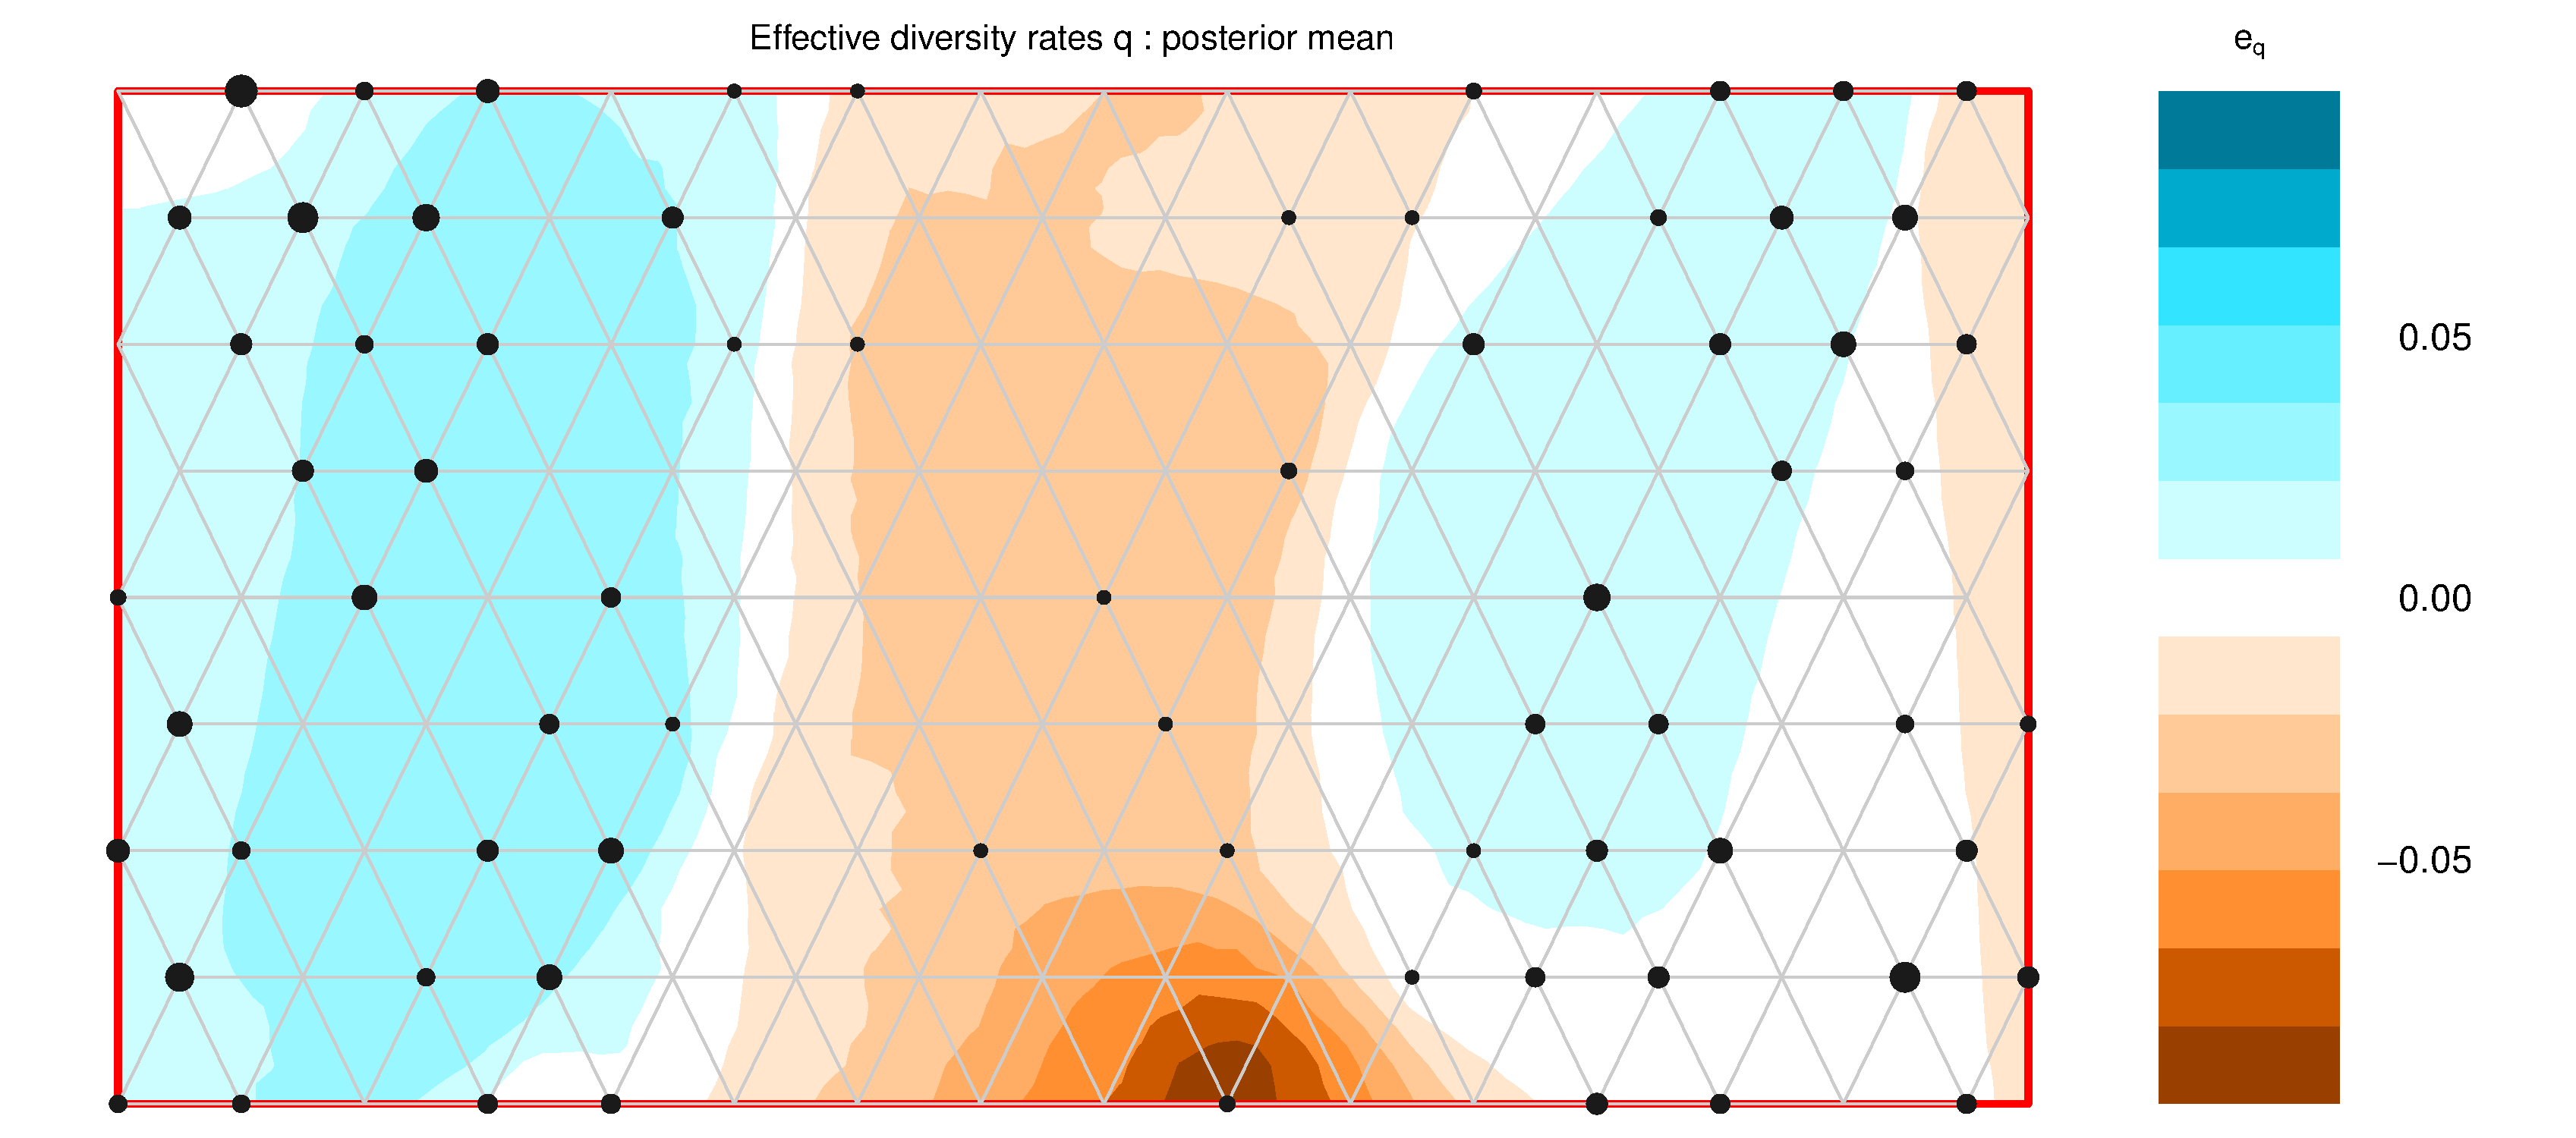
\includegraphics[height=2.4in]{barrier-schemeX-nIndiv300-nSites3000-EEMS-nDemes153-simno1_3-qrates01.png}
\caption{}
\end{subfigure}

\vspace{20pt}

\begin{subfigure}[t]{\textwidth}
\centering
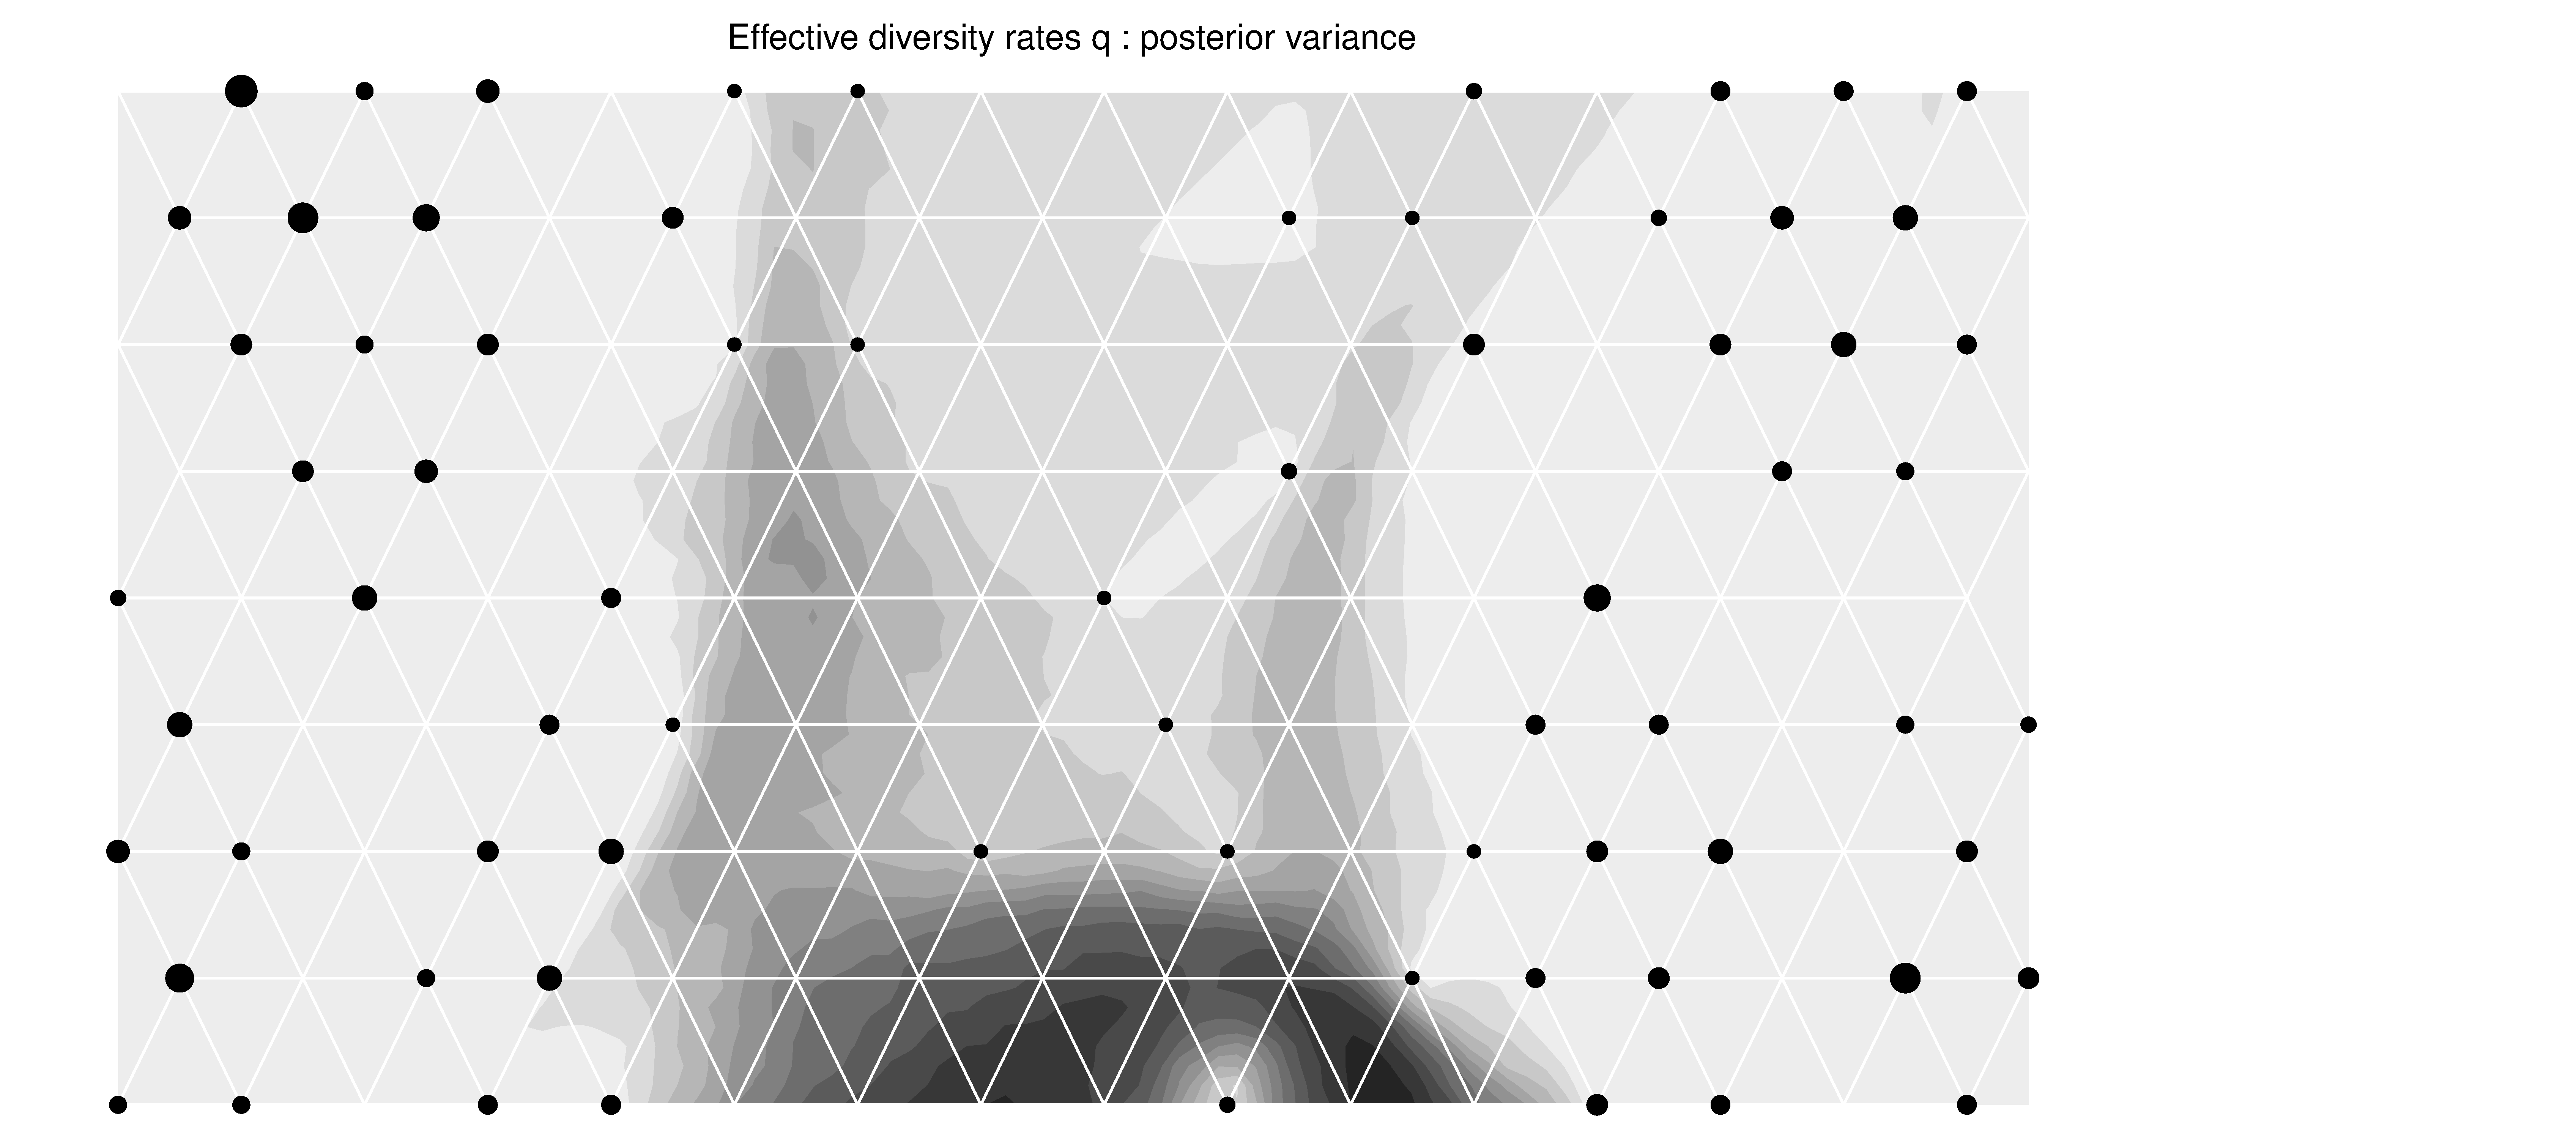
\includegraphics[height=2.4in]{barrier-schemeX-nIndiv300-nSites3000-EEMS-nDemes153-simno1_3-qrates02.png}
\caption{}
\end{subfigure}

\caption{EEMS analysis of a ``barrier to migration`` simulation. (a) Estimated effective diversity surface. (b) (Relative) Variance of the posterior mean diversity surface.}
\end{figure}
\clearpage}

\afterpage{
\begin{figure}[!]

\begin{subfigure}[t]{\textwidth}
\centering
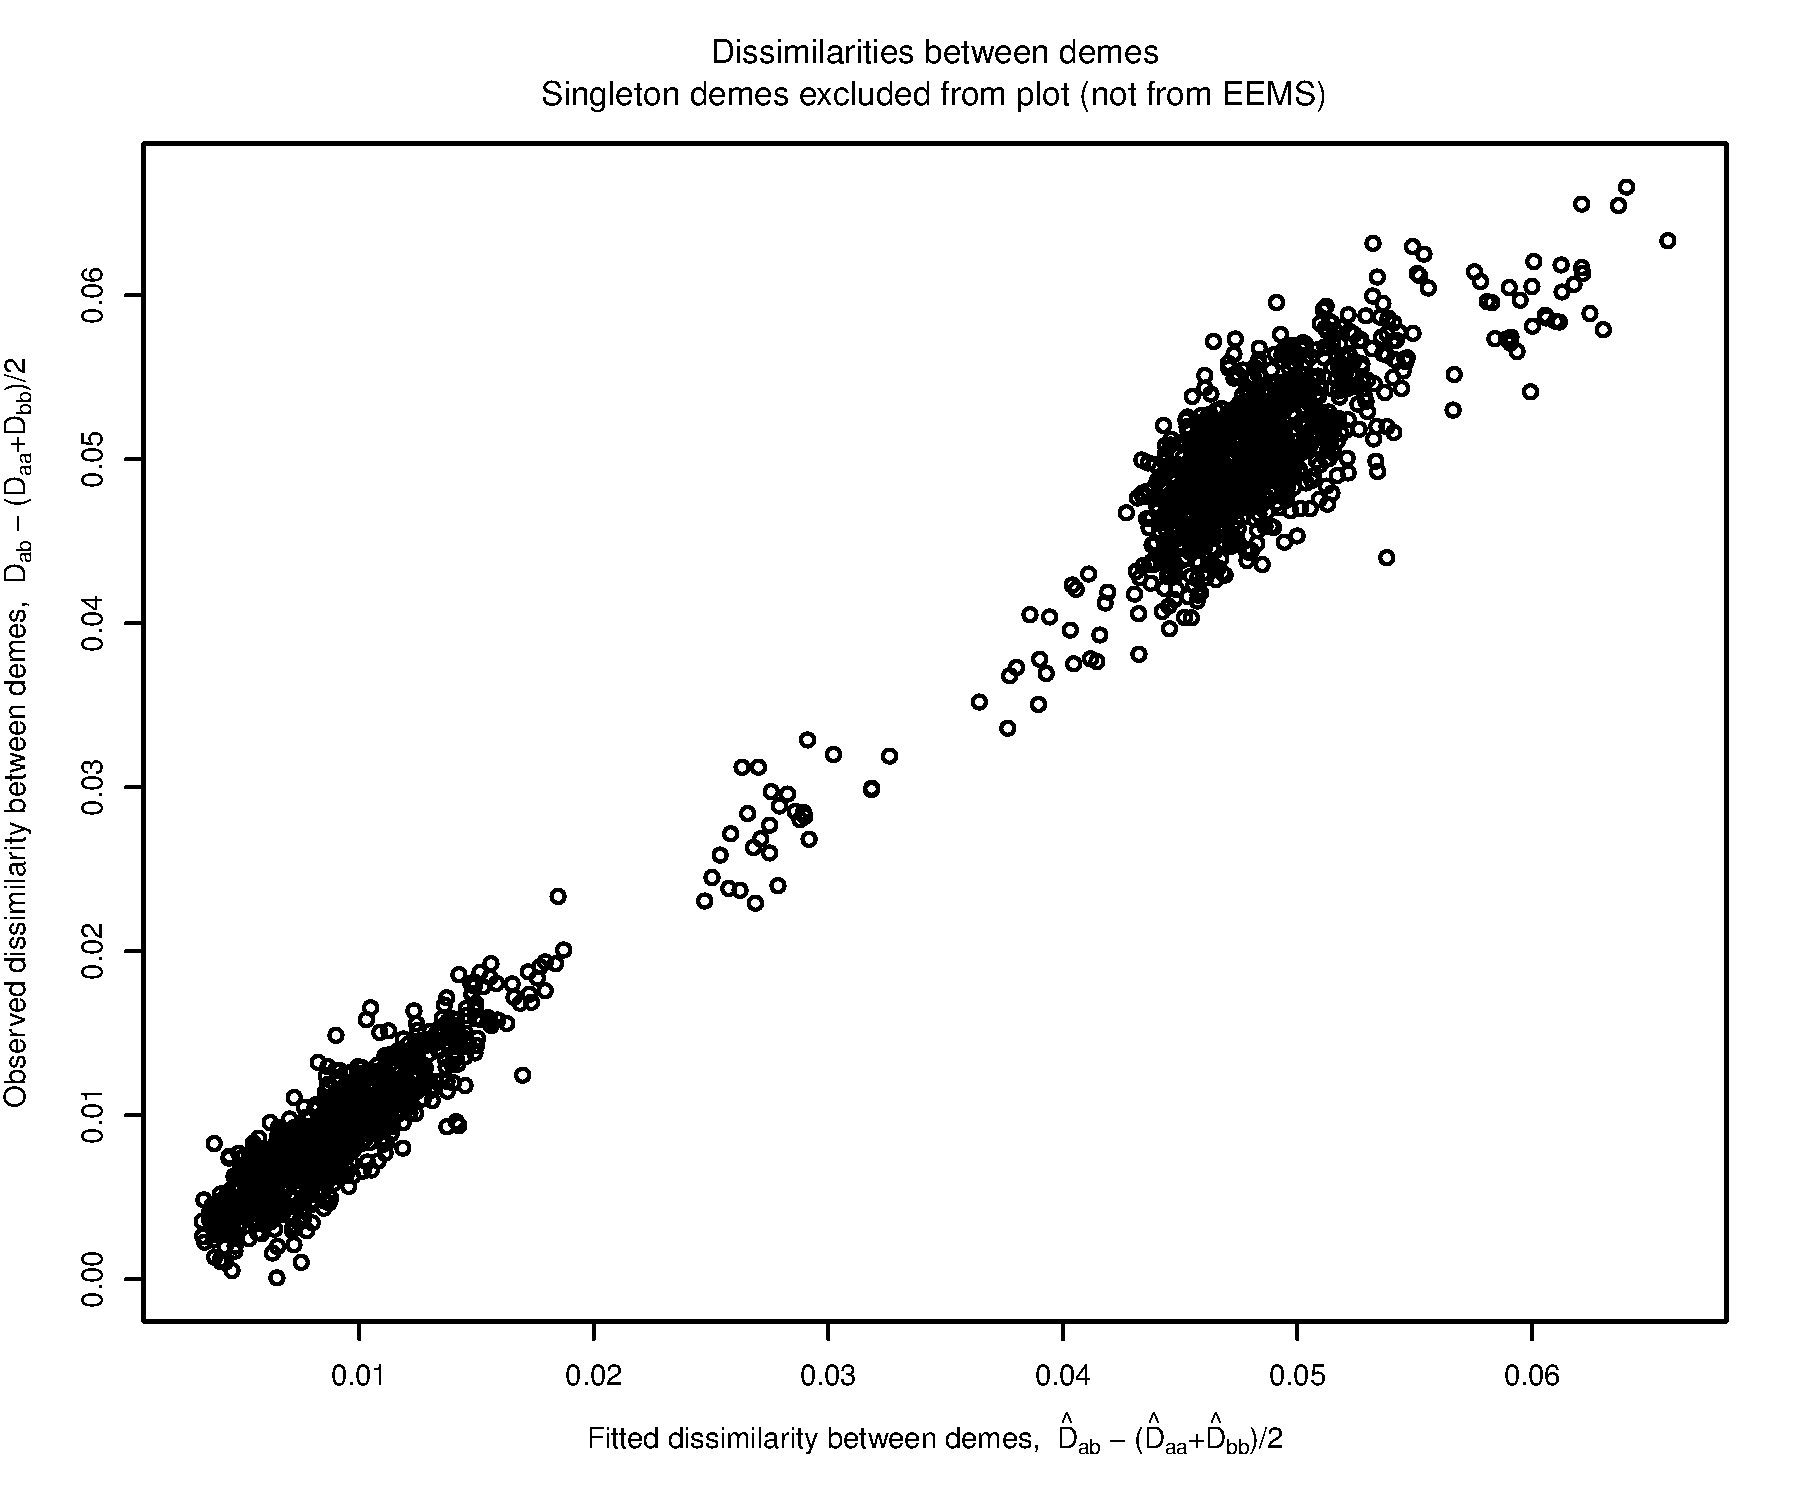
\includegraphics[height=3in]{barrier-schemeX-nIndiv300-nSites3000-EEMS-nDemes153-simno1_3-rdist01.png}
\caption{}
\end{subfigure}

\vspace{20pt}

\begin{subfigure}[t]{\textwidth}
\centering
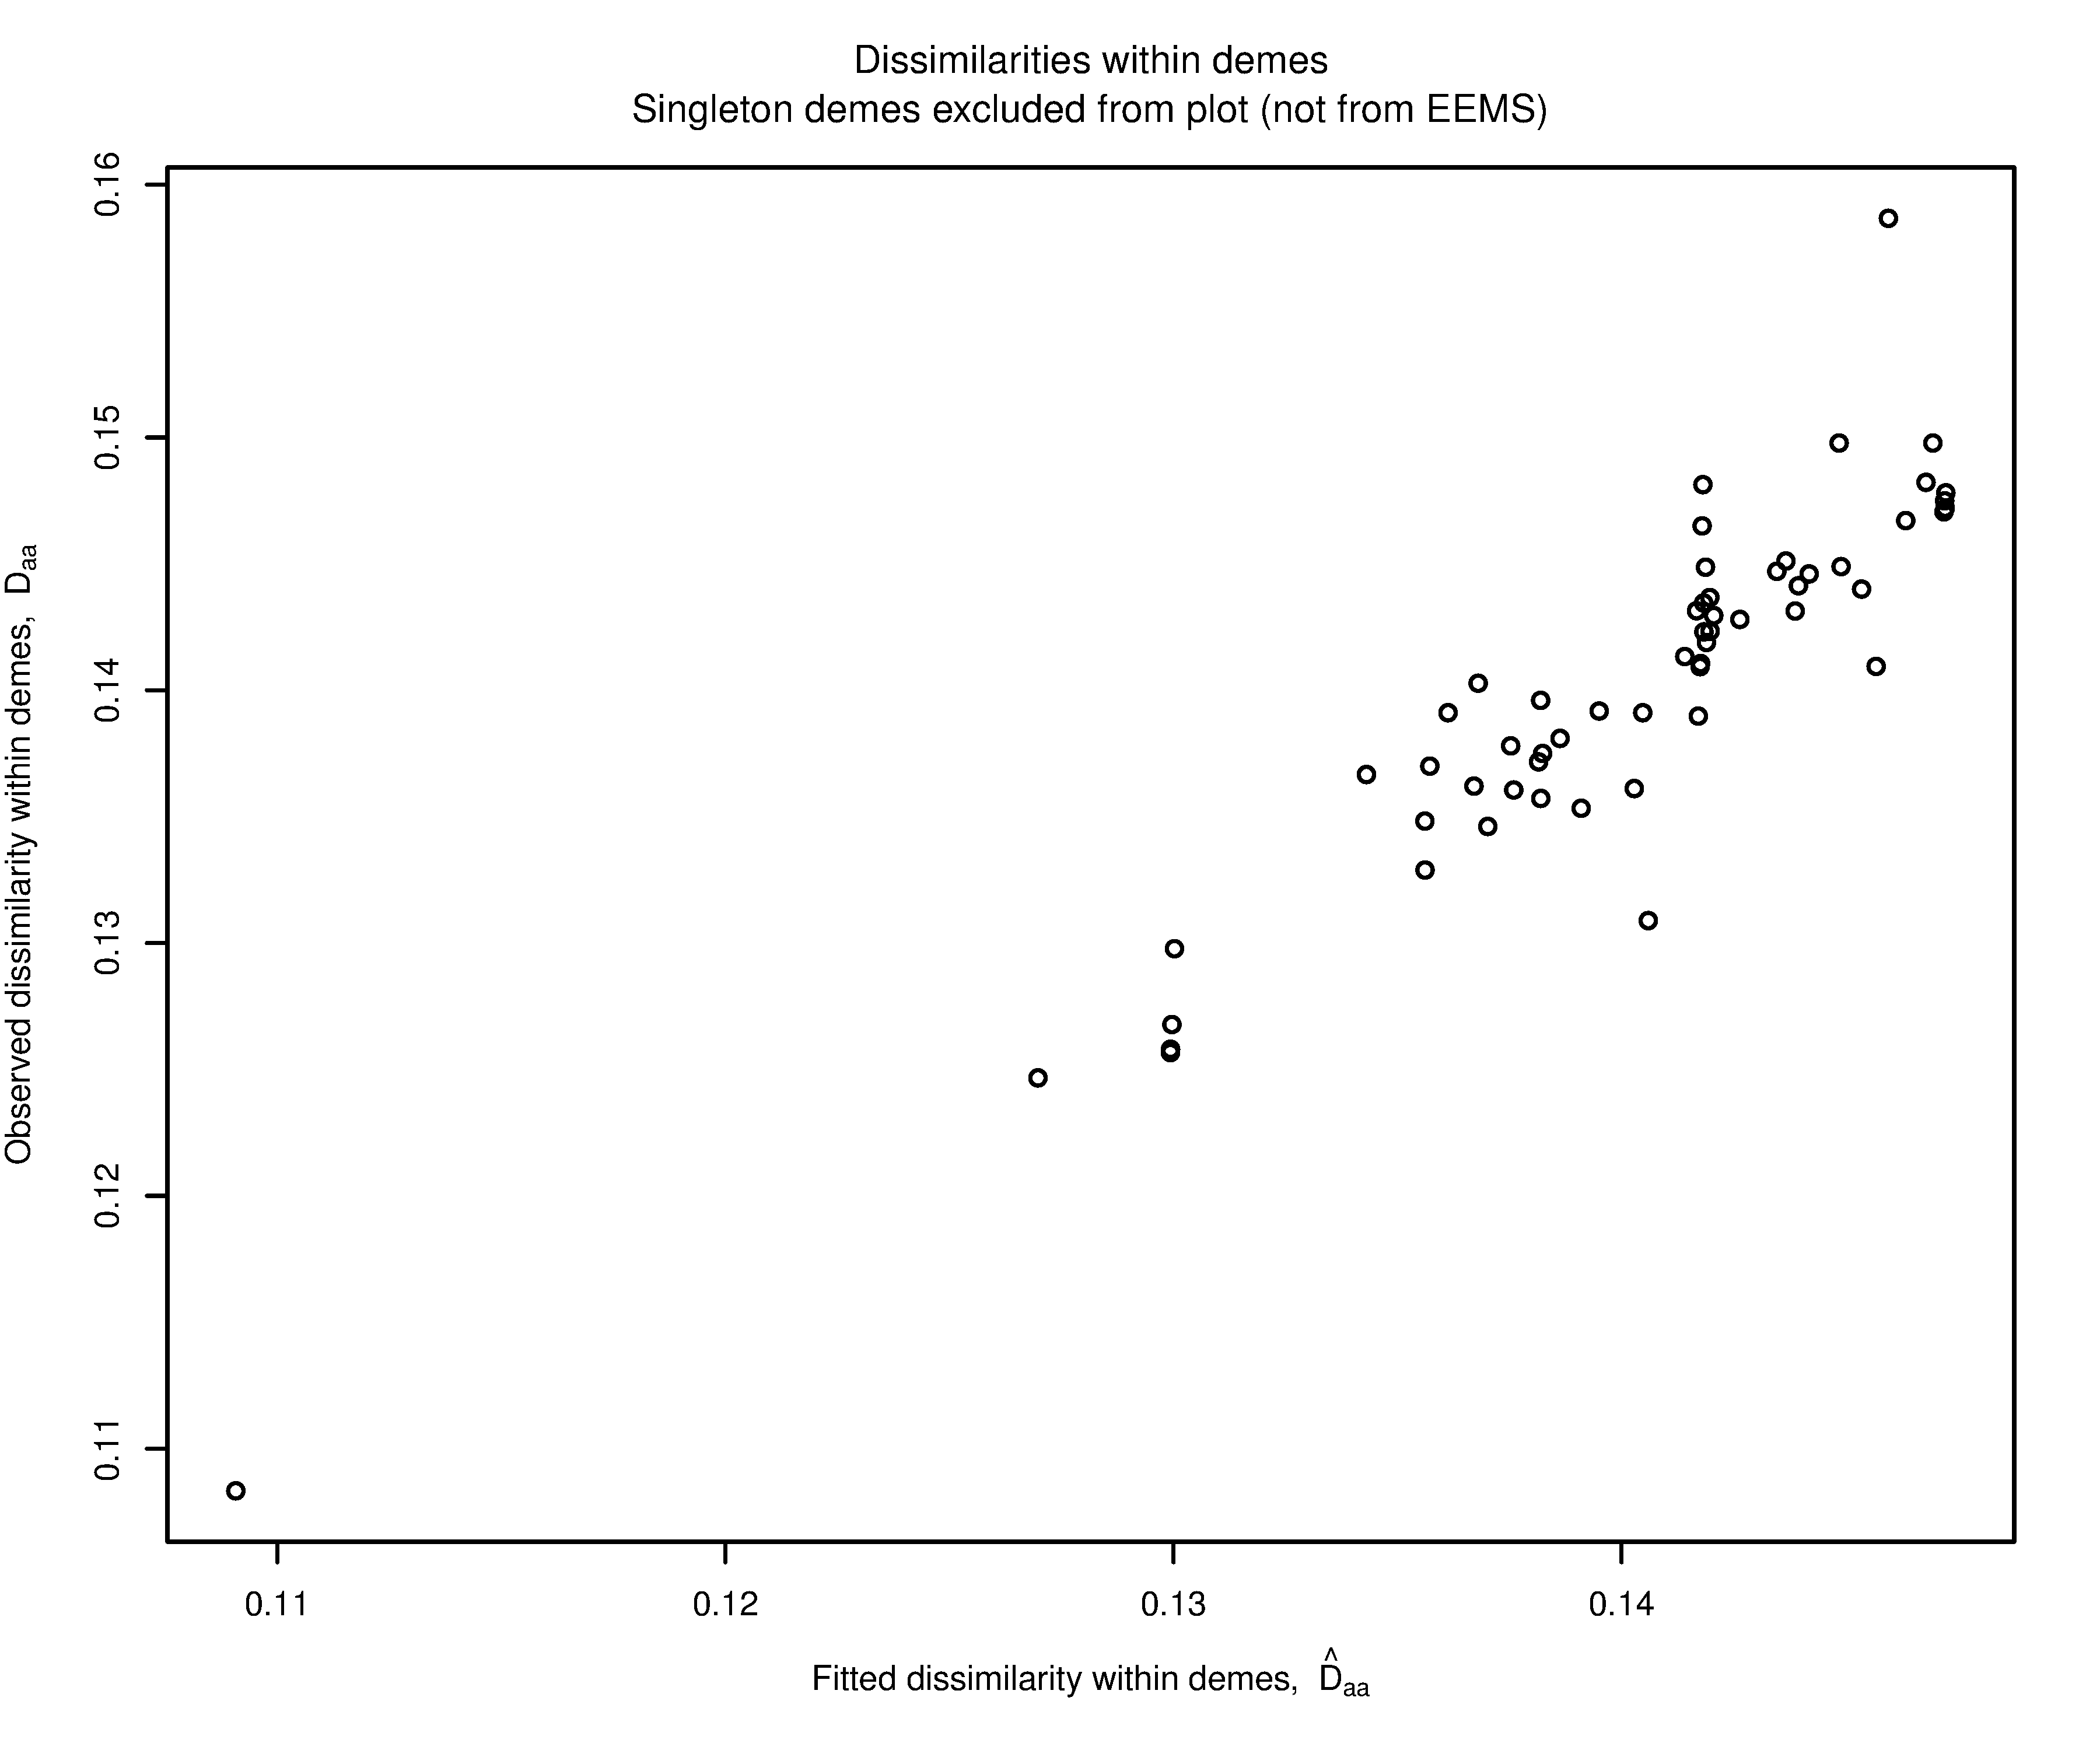
\includegraphics[height=3in]{barrier-schemeX-nIndiv300-nSites3000-EEMS-nDemes153-simno1_3-rdist02.png}
\caption{}
\end{subfigure}

\caption{Observed vs fitted genetic dissimilarities. (a) Dissimilarities between demes: $D_{\alpha\beta}-(D_{\alpha\alpha}+D_{\beta\beta})/2$. (b) Dissimilarities within demes: $D_{\alpha\alpha}$.}
\end{figure}
\clearpage}

\end{document}
